% Template Appunti Universitari %
\documentclass[12pt]{article}
\usepackage{graphicx} % Per inserire immagini
\usepackage{amsmath}  % Per formule matematiche avanzate
\usepackage{amssymb}  % Simboli aggiuntivi
\usepackage{geometry} % Margini più comodi
\geometry{margin=2.5cm}
\usepackage{parskip} % Rimuove l'indentazione e aggiunge spazio tra i paragrafi
\usepackage{hyperref} % Per i collegamenti ipertestuali
\usepackage{xcolor}
\usepackage{float}
\usepackage{fancyhdr} % Per modificare la numerazione e intestazioni
\usepackage{wrapfig} % aggiungi questo


\begin{document}

% ------------------------
% Titolo centrato verticalmente
% ------------------------
\thispagestyle{empty} % No page number
\vspace*{\fill}
\begin{center}
  {\LARGE \textbf{Industrial and\\ Collaborative Robotics\\[0.5em] (Part I)}}\\[1.5em]
  {\large Riccardo Florio}\\[0.5em]
  {\large May 2025}
\end{center}
\vspace*{\fill}
\newpage

% Pagina vuota
\thispagestyle{empty}
\mbox{}
\newpage

% ------------------------
% Indice (senza numero di pagina)
% ------------------------
\pagenumbering{gobble}
\tableofcontents
\newpage

% ------------------------
% Inizio della numerazione da 1
% ------------------------
\pagenumbering{arabic}
\setcounter{page}{1}

% ------------------------
% Inizio contenuto
% ------------------------

\section{Introduction}

\subsection{What is a robot?}

A robot is a \textbf{mechatronic system} designed to interact with its environment. It typically includes:
\begin{itemize}
  \item An \textbf{actuation system} to generate motion.
  \item A \textbf{sensing system} to acquire and process information about itself and the external world.
  \item A \textbf{control or AI system} to program and control its behavior.
\end{itemize}

A robot is therefore a \textbf{complex system} that embeds various technologies from mechanics, electronics, computer science, and artificial intelligence.

\begin{figure}[H]
  \centering
  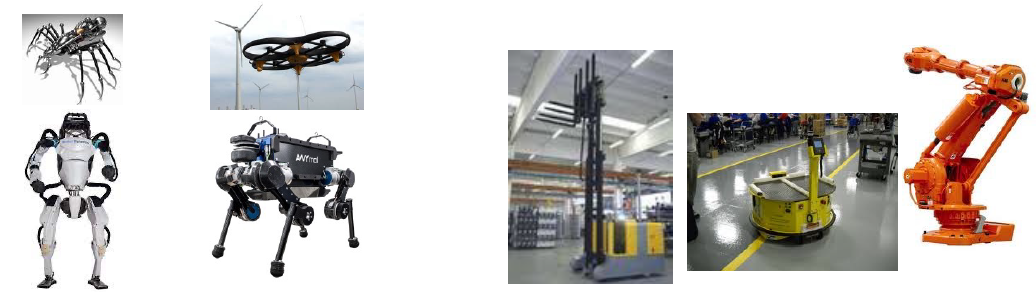
\includegraphics[width=\linewidth]{imgs/introduction_what_is_a_robot.png}
  \caption{Examples of different types of robots.}
\end{figure}

\hfill

\subsection{Robotics applications}

The first \textit{modern} robots were developed in the 1950s to support the teleoperation of radioactive materials and for prosthetic applications.

Robots began appearing in industrial environments in the 1970s, particularly in companies like General Motors. They were mainly employed for:
\begin{itemize}
  \item Welding
  \item Assembly
  \item Other repetitive and hazardous operations
\end{itemize}

Nowadays, robots are widely used in many other domains:
\begin{itemize}
  \item Medicine
  \item Space
  \item Military
  \item Entertainment
  \item \dots
\end{itemize}

\hfill

\subsection{Industrial Robotic Arms}

Industrial robotic arms are widely used in manufacturing and production lines. They are designed to perform specific, repetitive tasks with high precision and speed.

Typical applications include:
\begin{itemize}
  \item Mechanics
  \item Painting
  \item Placements
  \item Measurement control
\end{itemize}

\hfill
\begin{figure}[H]
  \centering
  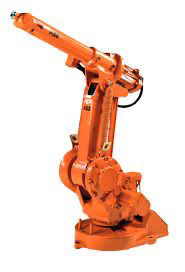
\includegraphics[width=0.2\linewidth]{imgs/industrial_robot_arm.png}
  \caption{Examples of different types of robots.}
\end{figure}

\hfill

\subsection{Industrial robotics}

In traditional industrial applications, robotic arms are employed for tasks that require:
\begin{itemize}
  \item High precision
  \item High repeatability
  \item High payload capacity
\end{itemize}

To guarantee safety, industrial robots are typically enclosed within physical barriers such as fences, preventing human access during operation.

Moreover, these robots are usually painted in bright colors to alert and warn operators of potential hazards in the workspace.

\hfill

\subsection{Advanced perception}

Advanced perception is a key component in modern robotics, especially within industrial robotic cells. Among all sensors, vision sensors are the most frequently used.

The main types of vision sensors include:
\begin{itemize}
  \item \textbf{Cameras}, which capture 2D images and video.
  \item \textbf{3D vision sensors}, which provide depth perception and spatial understanding.
\end{itemize}

These tools are essential for enabling robots to detect, recognize, and interact with objects in their environment.

\begin{figure}[H]
    \centering
    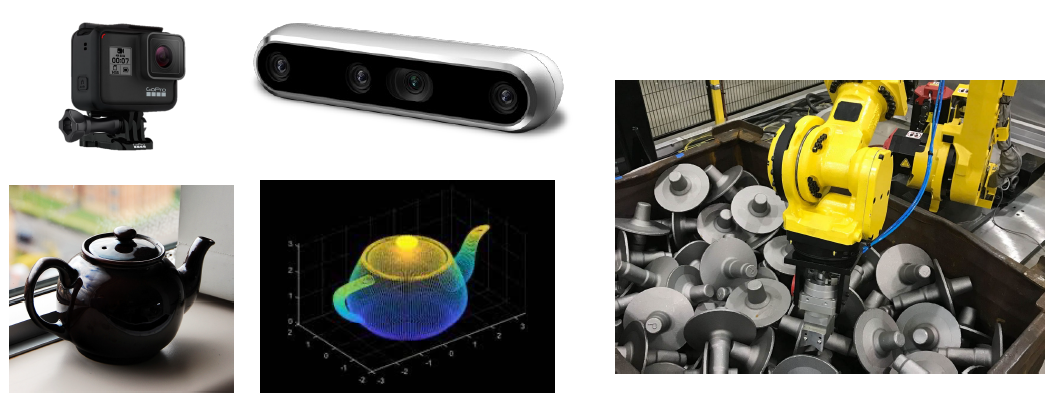
\includegraphics[width=\linewidth]{imgs/advanced_perception_sensors.png}
    \caption{Advanced perception sensors examples}
\end{figure}

\hfill

\subsection{Collaborative Robotics}

Collaborative robotics refers to systems where humans and robots operate together in a shared workspace.

Key features:
\begin{itemize}
  \item Human(s) and robots collaborate in the same area.
  \item No physical barriers are present between them.
\end{itemize}

\hfill
\begin{figure}[H]
    \centering
    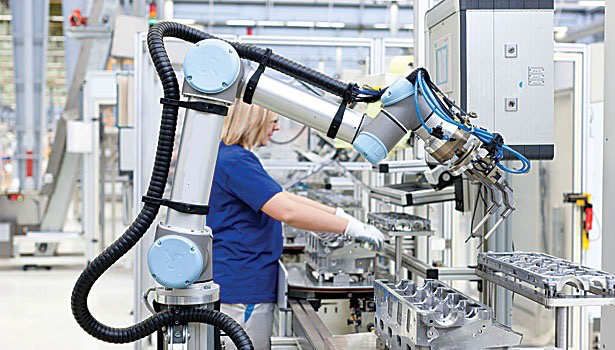
\includegraphics[width=0.6\linewidth]{imgs/collaborative_robotics_example.png}
    \caption{Collaborative robotics example}
\end{figure}

\hfill

\subsection{Collaboration}

There are various types of human-robot interaction, depending on the goal and the nature of the task.

The main distinctions are based on:
\begin{itemize}
  \item The proximity between the human and the robot (e.g., wearable, in-hand, arm's length, or out of reach).
  \item The frequency and level of interaction, which relate to the robot's agency.
\end{itemize}

These categories range from wearable robotics and teleoperated devices to highly interactive systems such as cooperative, collaborative, and supportive robots.

\begin{figure}[H]
  \centering
  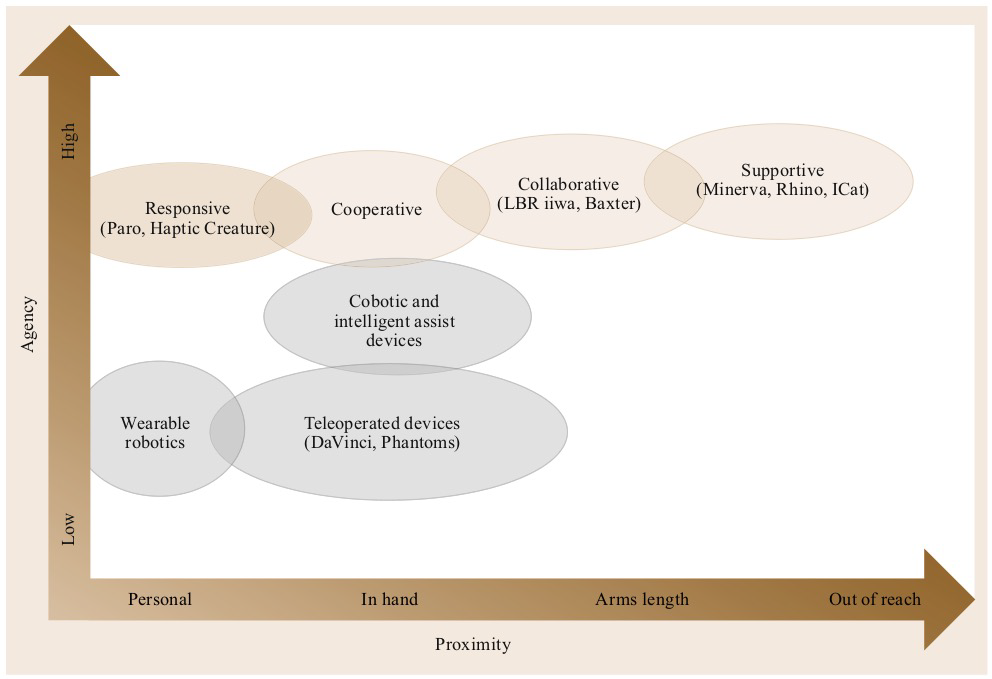
\includegraphics[width=\linewidth]{imgs/hri_interaction_types.png}
  \caption{Different types of human-robot interaction based on agency and proximity [Siciliano2016].}
\end{figure}

\hfill

\subsection{Supportive interaction}

In supportive interaction, the robot does not play the main role in the task. Instead, it supports the human operator by providing tools, materials, or information to enhance performance or help achieve specific objectives.

Examples include:
\begin{itemize}
  \item Museum guides
  \item Assistive robots
\end{itemize}

Safety is typically not an issue in this scenario because physical contact between the robot and the human rarely occurs. Furthermore, proximity control mechanisms are used to avoid unintended interactions.

\hfill

\subsection{Collaborative interaction}

In collaborative interaction, humans and robots work together on a task in a coordinated but separate manner. Each participant performs the part of the task that best suits their specific skills.

Some types of interaction are foreseen, such as:
\begin{itemize}
  \item Tool handover between robot and human
  \item Physical contact used intentionally to change the robot’s mode of operation (e.g., pushing the robot)
\end{itemize}

\hfill

\subsection{Cooperative interaction}

Cooperative interaction involves the human and robot jointly manipulating an object, leading to inevitable physical contact.

In this mode, both human and robot operate in direct contact—or through a shared object—with continuous shared control of the task execution.

This form of interaction is employed in scenarios such as:
\begin{itemize}
  \item Kinesthetic teaching
  \item Lifting and transportation
  \item Collaborative assembly
  \item Rehabilitation
\end{itemize}

\hfill

\subsection{Industrial Robotics: market data}

The annual installations of industrial robots have grown significantly over the last decade, reaching over 500,000 units worldwide in 2021.

\begin{figure}[H]
  \centering
  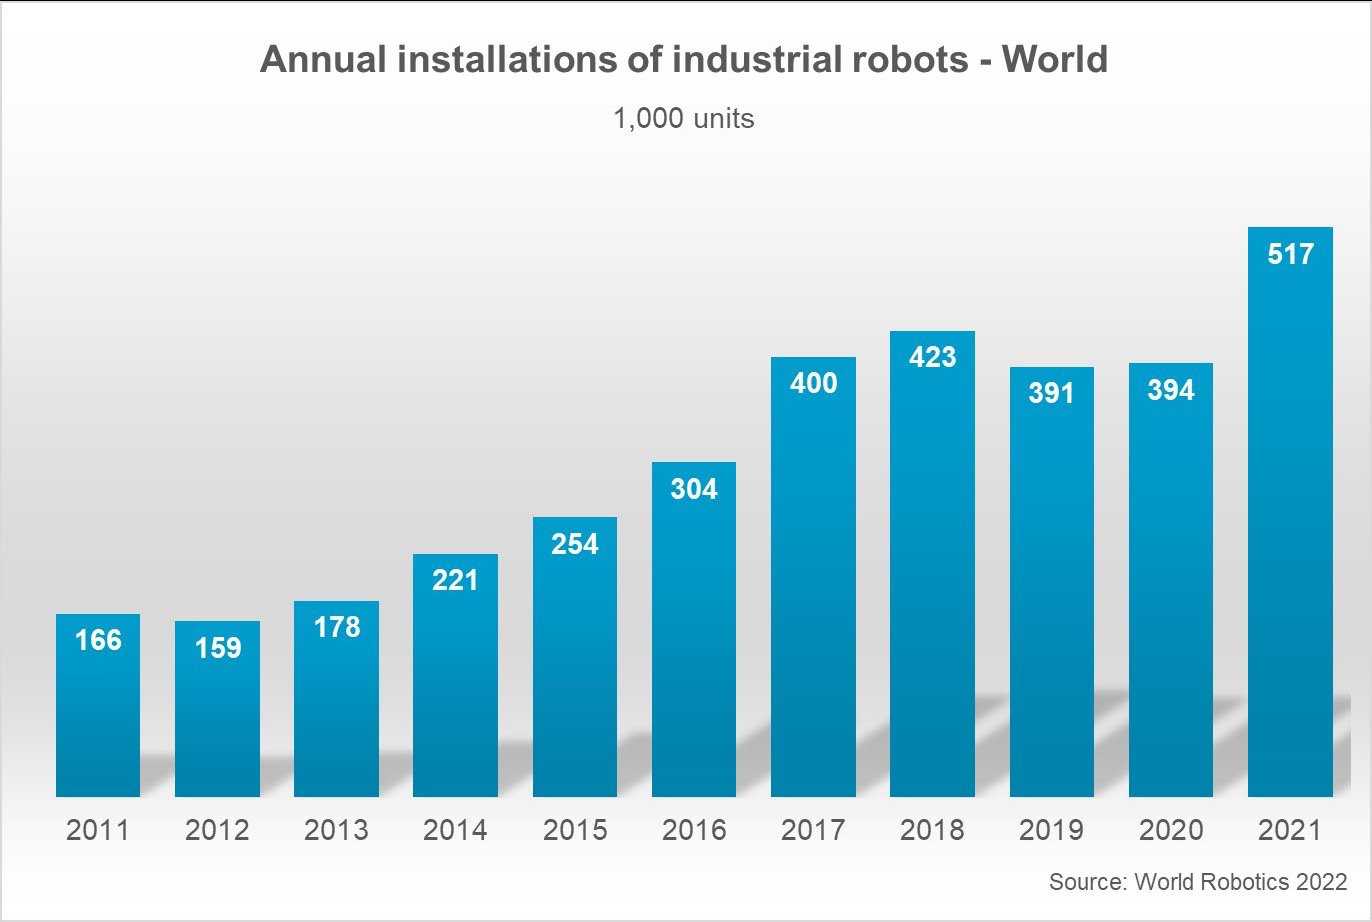
\includegraphics[width=0.85\linewidth]{imgs/industrial_robotics_world_installations.png}
  \caption{Annual installations of industrial robots worldwide (Source: World Robotics 2022).}
\end{figure}

The most demanding industries for industrial robots are electronics, automotive, and metal/machinery.

\begin{figure}[H]
  \centering
  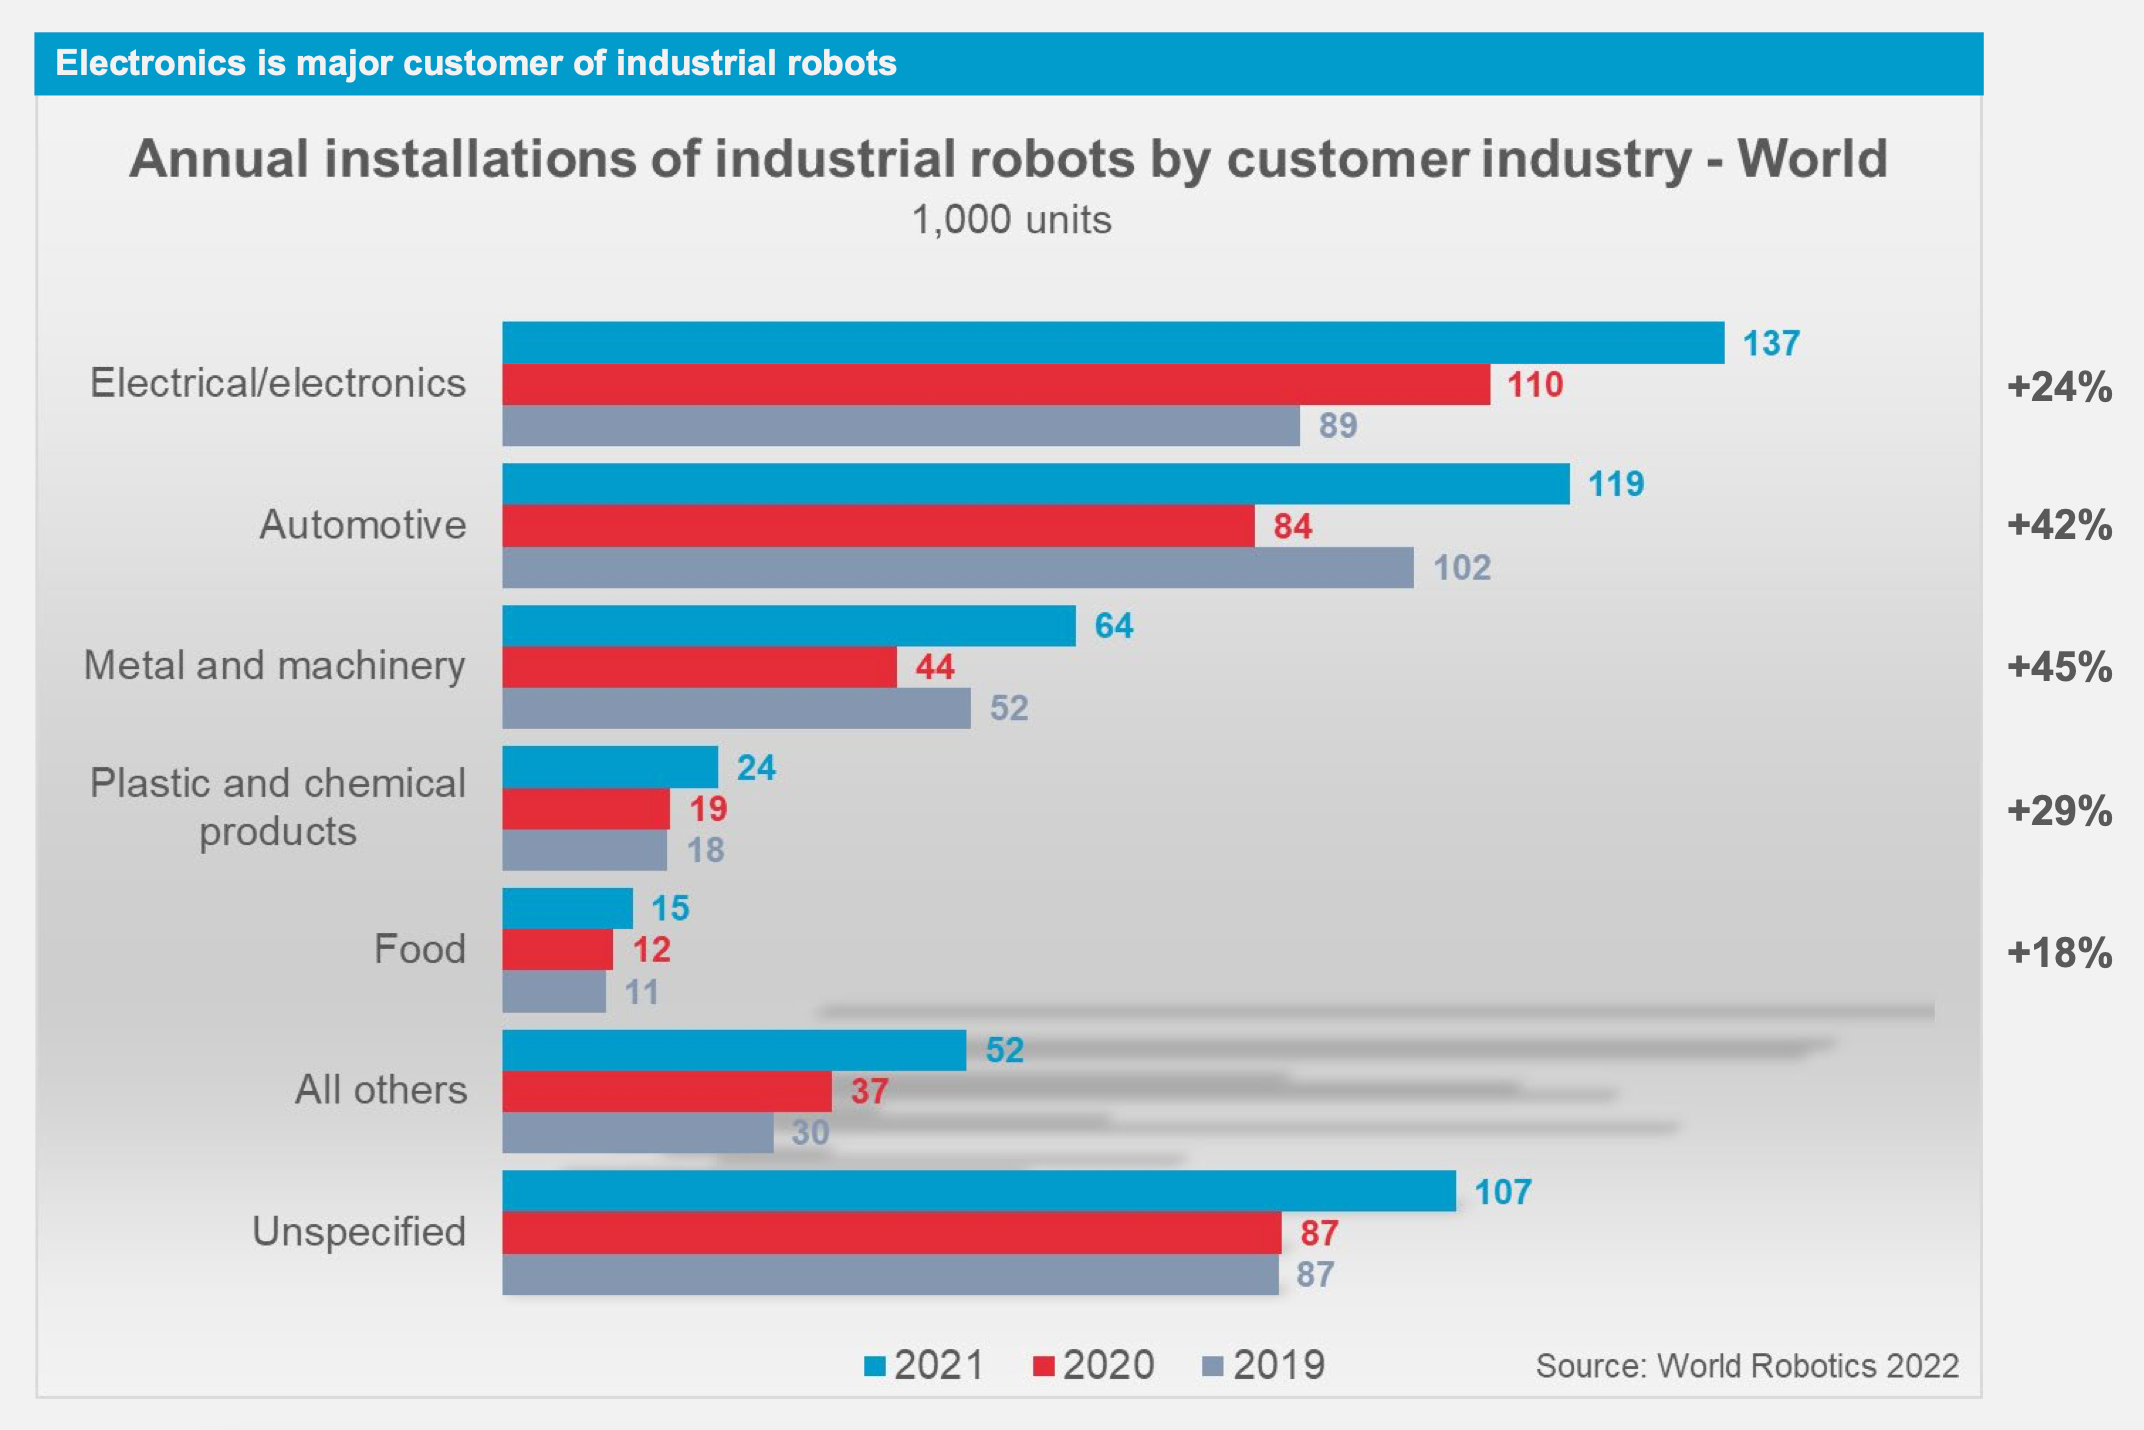
\includegraphics[width=0.85\linewidth]{imgs/industrial_robotics_by_industry.png}
  \caption{Robot installations by industry sector (Source: World Robotics 2022).}
\end{figure}

\hfill

\subsection{Industrial vs Collaborative Robotics}

Collaborative robots are still a small portion of total installations but are steadily growing, reaching 39,000 units in 2021 with a 50\% increase compared to the previous year.

\begin{figure}[H]
  \centering
  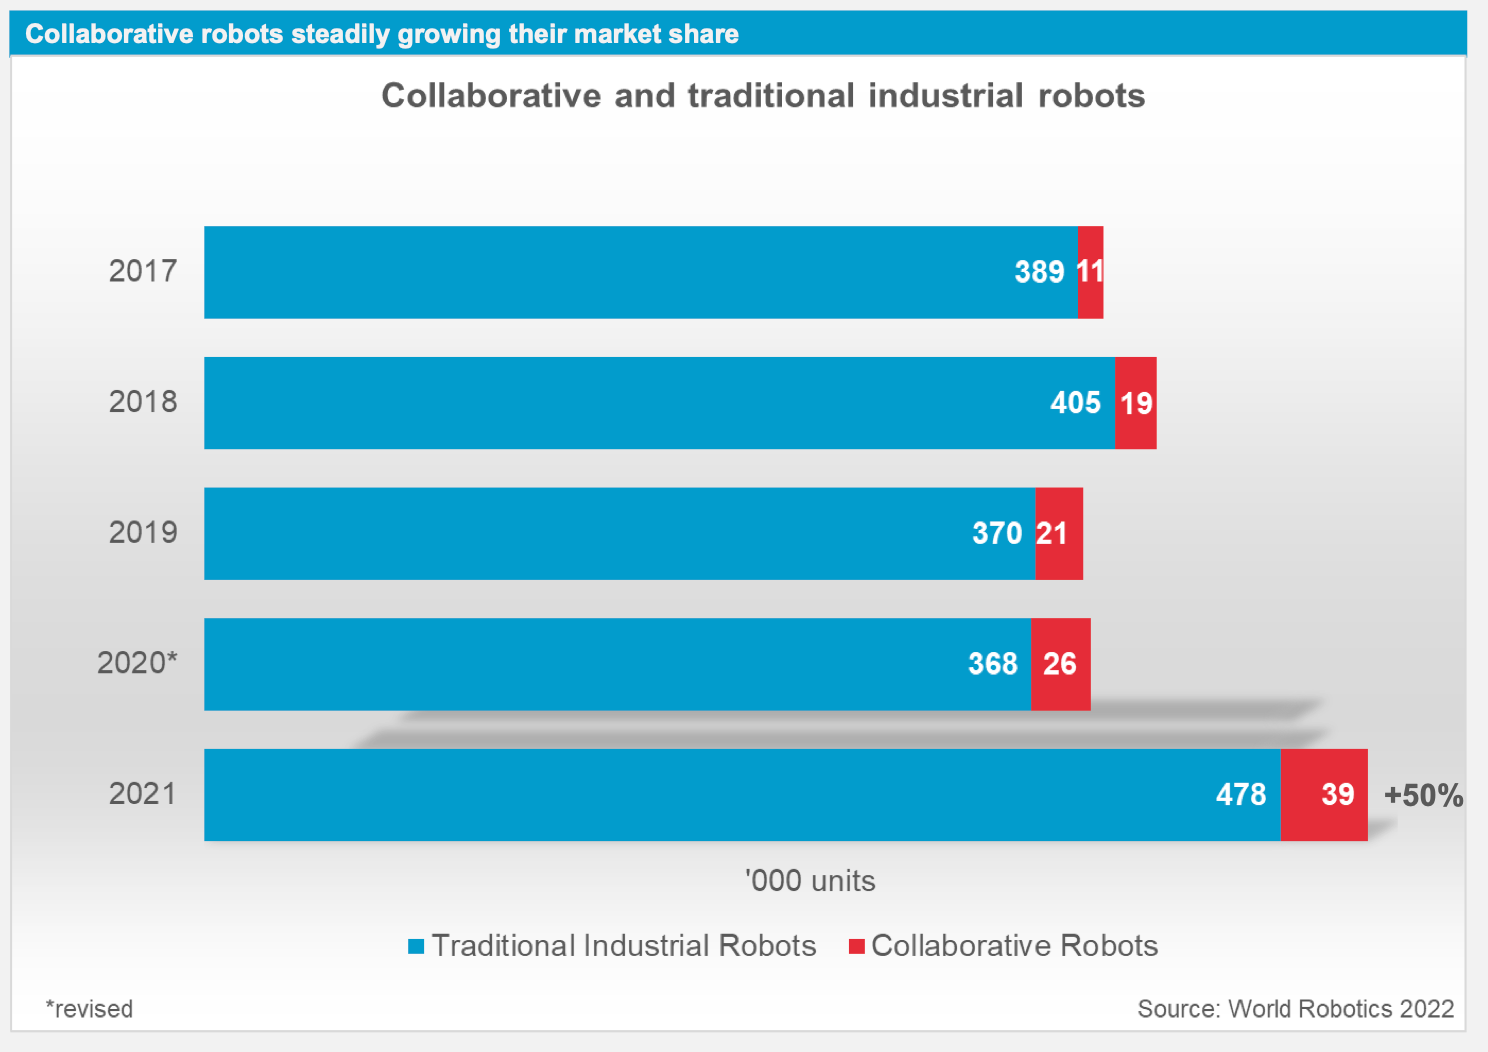
\includegraphics[width=0.85\linewidth]{imgs/industrial_vs_collaborative_robots.png}
  \caption{Comparison between industrial and collaborative robot installations (Source: World Robotics 2022).}
\end{figure}

\hfill

\subsection{Robotics in the World}

China leads the global robotics market by far, followed by Japan, the United States, and South Korea. Italy is in the top 5, with a significant growth rate of +65\%.

\begin{figure}[H]
  \centering
  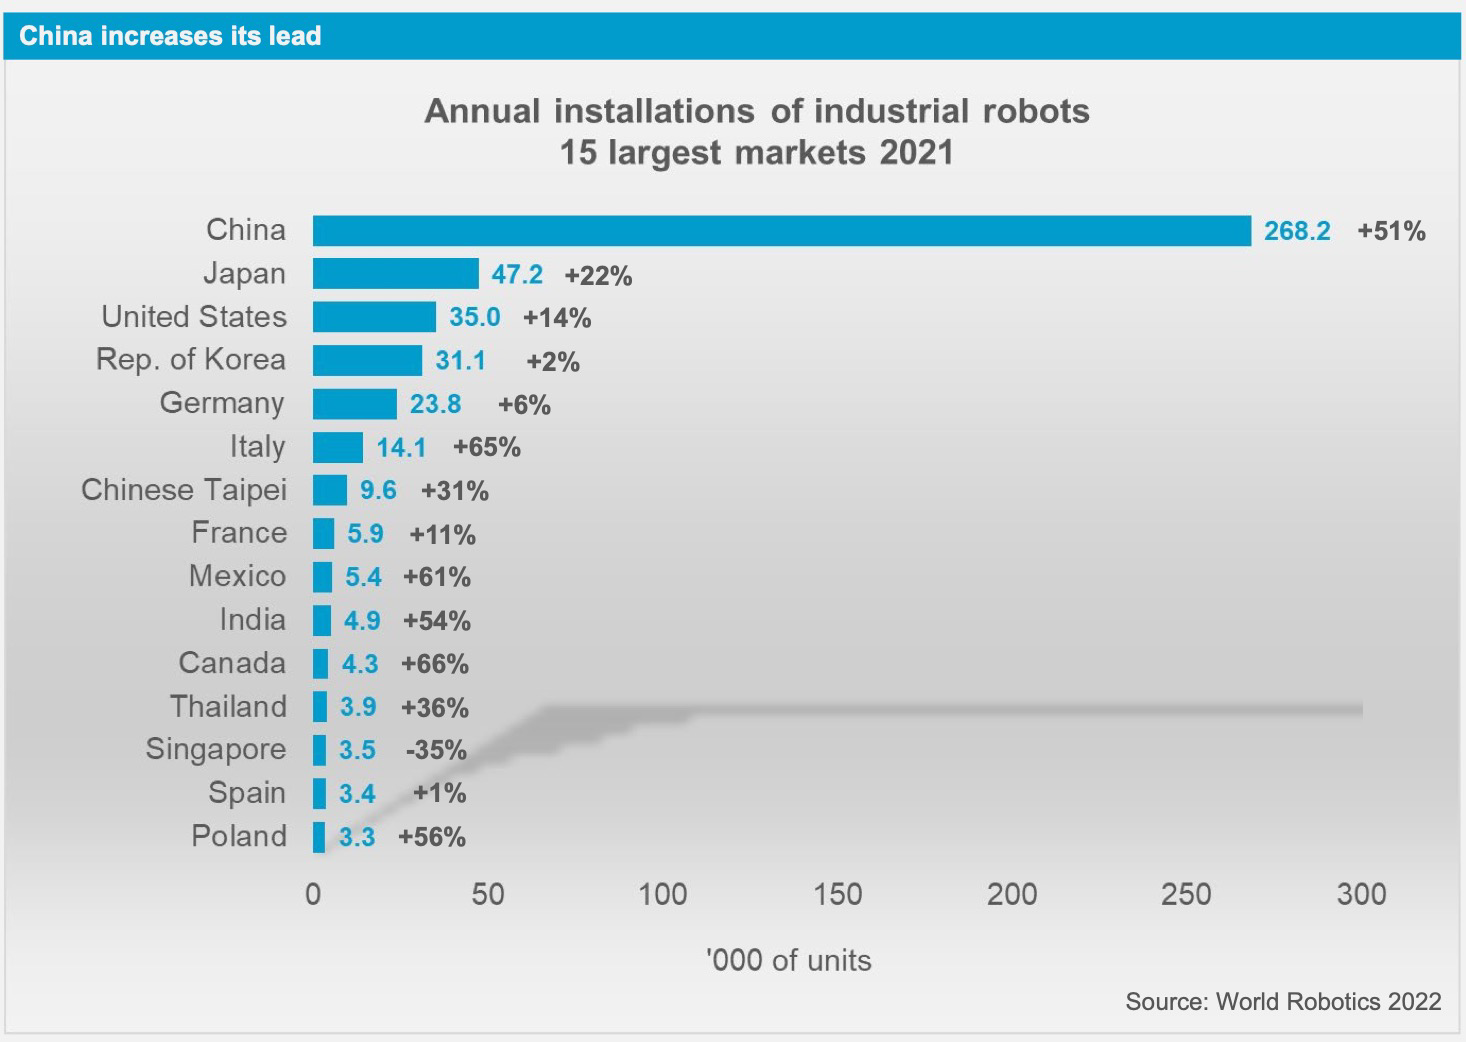
\includegraphics[width=0.85\linewidth]{imgs/robotics_by_country.png}
  \caption{Top 15 countries for robot installations in 2021 (Source: World Robotics 2022).}
\end{figure}

\newpage
\section{Robot Arms and Mobile Robots}

\subsection{What kind of robots are we considering}

In this course, we consider two main categories of robots:
\begin{itemize}
  \item \textbf{Robotic arms}: these are stationary manipulators used for tasks like welding, painting, assembling, etc.
  \item \textbf{Mobile robots}: these include autonomous ground vehicles used for transporting goods or navigating in industrial environments.
\end{itemize}

Both categories may belong to either of the following types:
\begin{itemize}
  \item \textbf{Collaborative robots (cobots)}: designed to work safely alongside humans without fencing or physical barriers.
  \item \textbf{Non-collaborative robots}: typically operate in isolated or restricted areas due to safety concerns.
\end{itemize}

\begin{figure}[H]
  \centering
  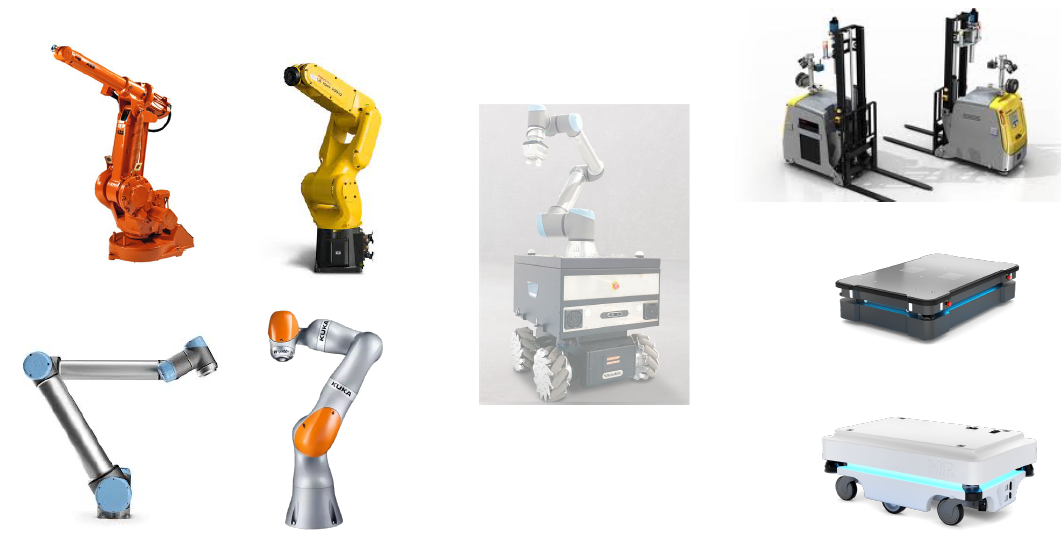
\includegraphics[width=\linewidth]{imgs/robot_types.png}
  \caption{Examples of robotic arms (top left), collaborative arms (bottom left), mobile robots (right), and integrated mobile manipulators (center).}
\end{figure}

\hfill

\subsection{Robotic Arms}

A robotic system is composed of two main components:

\begin{itemize}
  \item \textbf{The control system}: this is the electronic part responsible for processing commands, executing motion planning, and interfacing with the environment and the user. It includes the \textbf{teach-pendant}, a handheld device used by operators to program and manually control the robot.
  \item \textbf{The manipulator}: this is the mechanical structure of the robot—often an articulated arm—used to physically interact with the environment by performing tasks like moving, gripping, or assembling objects.
\end{itemize}

These two parts are strongly interconnected and operate together to enable robotic functionality.

\begin{figure}[H]
  \centering
  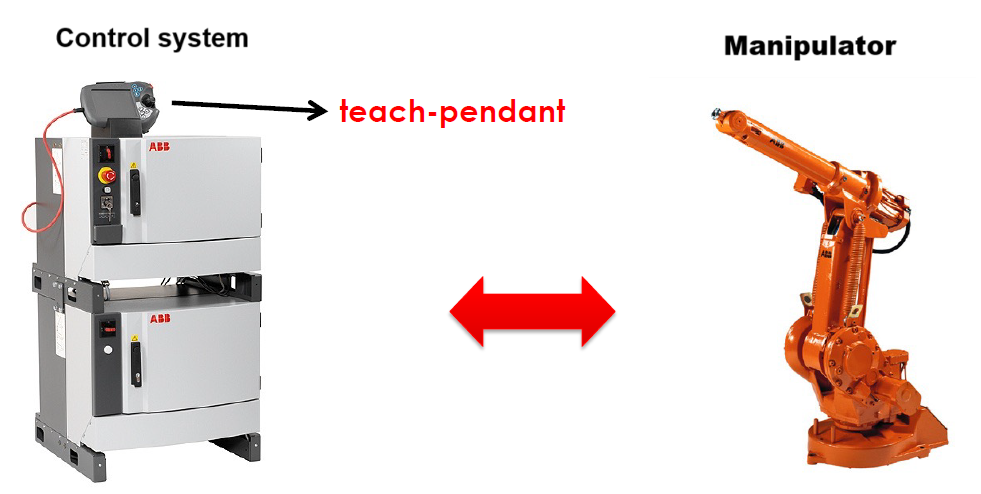
\includegraphics[width=0.7\linewidth]{imgs/robotic_arm_structure.png}
  \caption{Composition of a robot: the control system (left, with teach-pendant) and the mechanical manipulator (right).}
\end{figure}

\hfill

\subsection{The control system}

The control system is considered the \textbf{``brain''} of the robot. Its main role is to determine the motions that the manipulator should perform, based on:
\begin{itemize}
  \item The assigned task;
  \item Information received from sensors;
  \item Internal control algorithms.
\end{itemize}

It is generally a \textbf{complex architecture}, composed of multiple processors and often connected to various devices for monitoring, control, and data storage.

The fundamental functions that every control system must implement are:
\begin{itemize}
  \item \textbf{Human interface}: to allow operators to interact with the robot, e.g., via a teach pendant;
  \item \textbf{Data storage}: for saving configurations, logs, and programs;
  \item \textbf{Motion planning}: to compute trajectories and motion sequences;
  \item \textbf{Real-time joint control}: to precisely actuate the robot in real-time;
  \item \textbf{Sensor monitoring}: to continuously read and react to sensor data.
\end{itemize}

\hfill

\subsection{The manipulator}

The manipulator is the part of the robot that directly interacts with the external environment. It is typically composed of:

\begin{itemize}
  \item A series of rigid bodies called \textbf{links};
  \item A series of actuated interconnections called \textbf{joints}.
\end{itemize}

The manipulator is anchored by a \textbf{base}, which can either be fixed to the ground or mounted on a mobile platform.

At the opposite end, the manipulator typically features an \textbf{end-effector}—the component that performs the actual work. Examples include:
\begin{itemize}
  \item Grippers;
  \item Welders;
  \item Hands or other tools.
\end{itemize}

The end-effector is mounted on the \textbf{wrist}, a joint that provides orientation and fine rotation capabilities to the tool.

\begin{figure}[H]
  \centering
  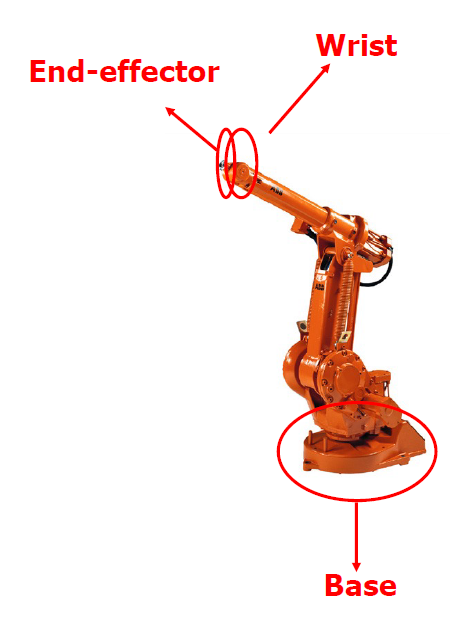
\includegraphics[width=0.35\linewidth]{imgs/manipulator_labeled.png}
  \caption{Main components of a robotic manipulator: base, wrist, and end-effector.}
\end{figure}

\subsection{Common mechanical structures for robotic arm}

Several mechanical structures can be adopted for building a robotic arm. The most common ones are:

\begin{itemize}
  \item \textbf{Cartesian configuration}: composed of three linear axes (X, Y, Z). It is suitable for tasks that require high precision and repeatability in a cuboidal workspace.
  \item \textbf{Cylindrical configuration}: includes one rotary joint at the base and two linear movements. It provides access to a cylindrical workspace.
  \item \textbf{SCARA configuration (Selective Compliance Articulated Robot Arm)}: designed primarily for horizontal movement, combining rotary and linear motions.
  \item \textbf{Anthropomorphic configuration (or articulated arm)}: resembles the human arm, with several rotary joints providing high flexibility and reachability.
\end{itemize}

\begin{figure}[H]
  \centering
  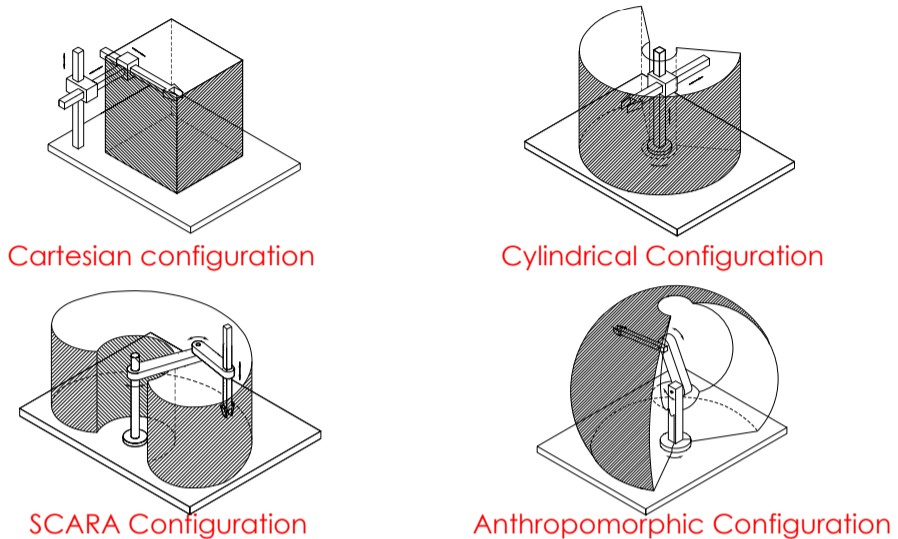
\includegraphics[width=0.8\linewidth]{imgs/mechanical_structures_schematic.png}
  \caption{Schematic representation of different mechanical configurations: Cartesian, Cylindrical, SCARA, and Anthropomorphic.}
\end{figure}

\begin{figure}[H]
  \centering
  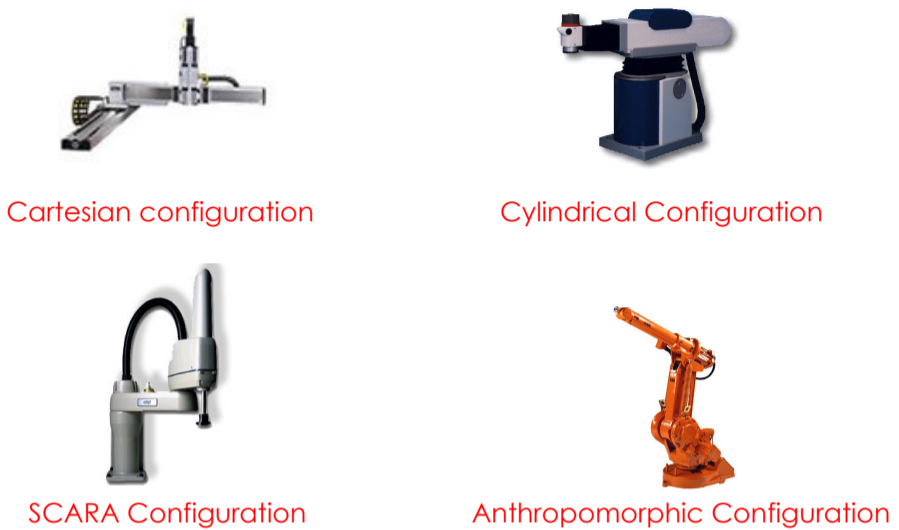
\includegraphics[width=0.8\linewidth]{imgs/mechanical_structures_real.png}
  \caption{Real-world examples of the same mechanical configurations.}
\end{figure}

Among these, the two most common configurations are the Cartesian and the Anthropomorphic ones:

\begin{itemize}
  \item The \textbf{Cartesian structure} is very robust and ideal for transporting heavy loads with high repeatability. However, it tends to be bulky and lacks dexterity.
  \item The \textbf{Anthropomorphic structure} is less robust and has lower payload capacity. Nevertheless, it is compact and offers high dexterity, enabling it to reach distant and complex positions.
\end{itemize}

\hfill

\subsection{Workspace}

The \textbf{workspace} (also called \textbf{task space}) of a robot is the set of all points that its end-effector can reach.

The shape and size of the workspace depend on:
\begin{itemize}
  \item The dimensions of the robot's links;
  \item The type and number of joints;
  \item The mobility limits of each joint.
\end{itemize}

Understanding the workspace is essential for determining the capabilities of a robot in performing tasks within its physical range.

\begin{figure}[H]
  \centering
  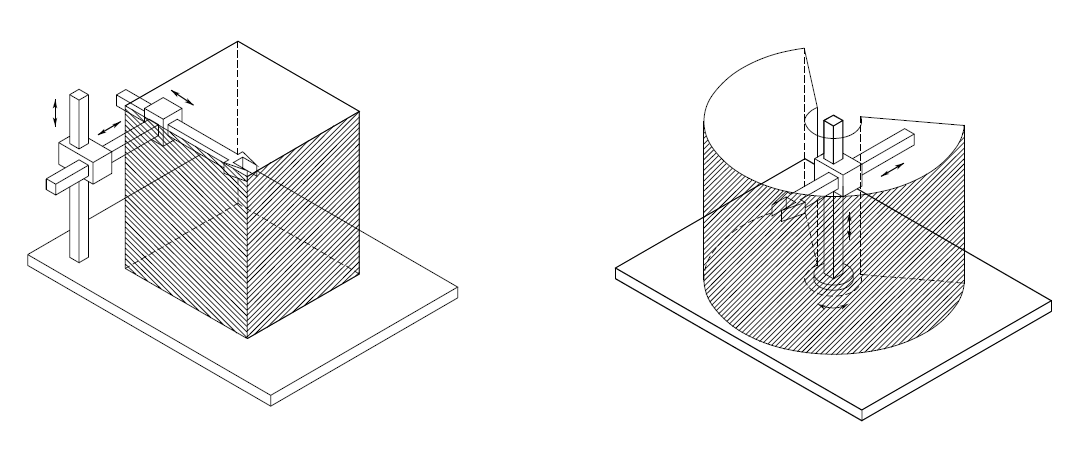
\includegraphics[width=0.85\linewidth]{imgs/workspace.png}
  \caption{Examples of workspace for Cartesian (left) and cylindrical (right) robot configurations.}
\end{figure}

\hfill

\subsection{Joints}

A \textbf{joint} allows a relative motion between two connected links in a robotic arm.

There are two primary types of joints:
\begin{itemize}
  \item \textbf{Prismatic joint} (T): allows linear translation between links;
  \item \textbf{Rotational joint} (R): allows angular rotation between links.
\end{itemize}

More complex joints—such as \textbf{spherical} or \textbf{helicoidal} joints—can be realized through combinations of rotational and/or prismatic joints.  
For instance, a spherical joint can be implemented using three intersecting rotational joints.

Mechanical configurations can also be identified by the sequence of joint types they use. Common notations include:

\begin{itemize}
  \item \textbf{TTT}: Three prismatic joints (Cartesian structure);
  \item \textbf{RT}: One rotational and one prismatic joint (Cylindrical structure);
  \item \textbf{RRT}: Two rotational and one prismatic joint (SCARA structure);
  \item \textbf{RRR}: Three rotational joints (Anthropomorphic structure).
\end{itemize}

\begin{figure}[H]
  \centering
  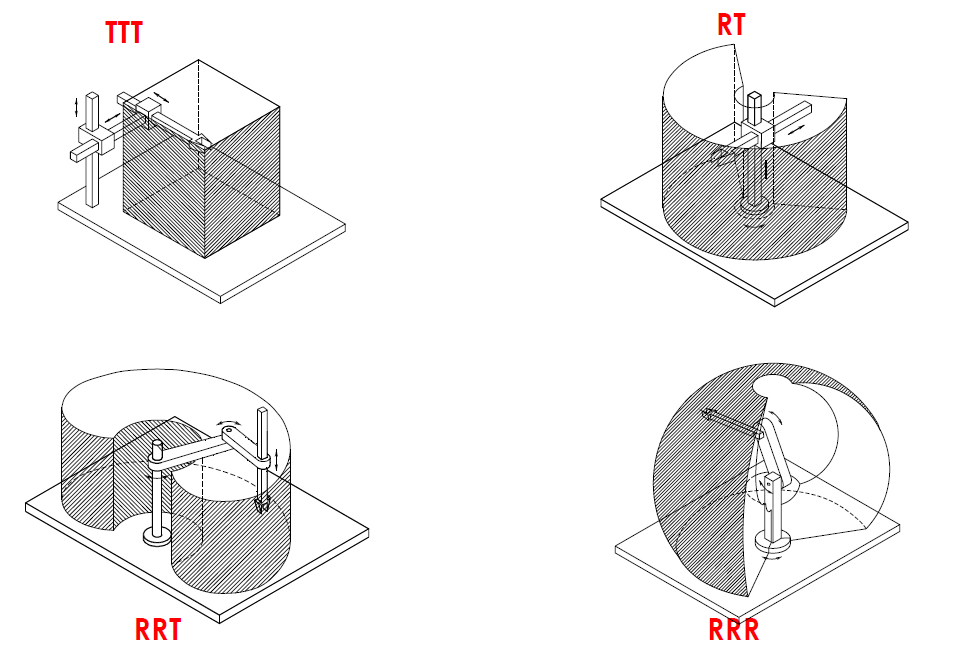
\includegraphics[width=0.8\linewidth]{imgs/joint_configurations.png}
  \caption{Joint configurations for common robot types: TTT, RT, RRT, and RRR.}
\end{figure}

\hfill

\subsection{Degrees of Freedom (DOFs) of a manipulator}

The \textbf{degrees of freedom (DOFs)} of a robotic arm correspond to the number of independent movements the robot can perform, which is typically equal to the number of joints.

\begin{itemize}
  \item For simple manipulators: DOFs = number of joints.
  \item For more complex mechanisms, DOFs can be calculated using the \textit{Gruebler formula}.
\end{itemize}

Intuitively, DOFs describe how the end-effector can move in space. The maximum DOFs required to fully control the position and orientation in 3D space is 6 (3 for translation, 3 for rotation).

Let $n$ be the number of joints and $m$ the dimension of the task space:
\begin{itemize}
  \item If $n = m$: the robot can reach any position and orientation — this is a fully controlled system.
  \item If $n < m$: the robot is \textbf{defective}, unable to cover the full workspace with all orientations.
  \item If $n > m$: the robot is \textbf{redundant}, offering multiple ways to reach the same point.
\end{itemize}

\begin{figure}[H]
  \centering
  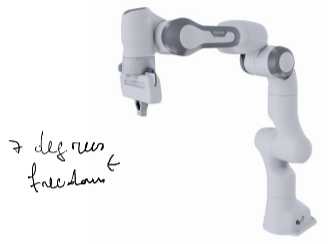
\includegraphics[width=0.4\linewidth]{imgs/franka_panda.png}
  \caption{Franka Emika Panda robot: an example of a redundant manipulator with 7 degrees of freedom.}
\end{figure}

\begin{figure}[H]
  \centering
  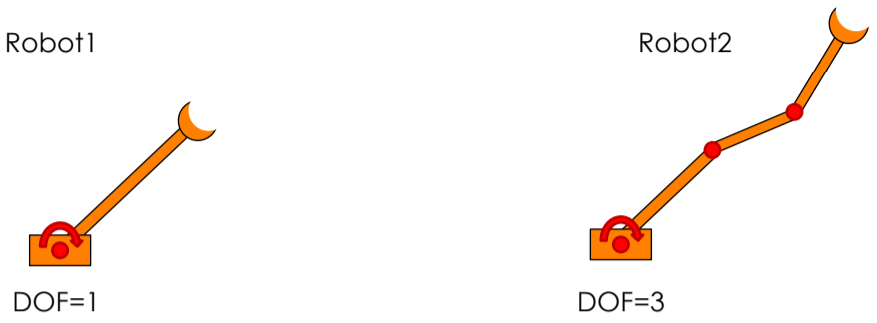
\includegraphics[width=0.8\linewidth]{imgs/dof_examples.png}
  \caption{Simple visual examples: Robot1 with 1 DOF and Robot2 with 3 DOFs.}
\end{figure}

\hfill

\subsection{Joint space and Workspace}

Each joint in a robot is actuated, meaning it is possible to independently control its position. 

To each joint is associated a \textbf{joint variable} $q_i$, which defines the relative position of the $i$-th link with respect to the previous one.

The set of all possible combinations of joint variables defines the \textbf{joint space} of the robot.

In general, if a robot has $n$ joints, its joint space is:
\[
q = 
\begin{pmatrix}
q_1 \\
\vdots \\
q_n
\end{pmatrix}
\in \mathbb{R}^n
\]

\begin{figure}[H]
  \centering
  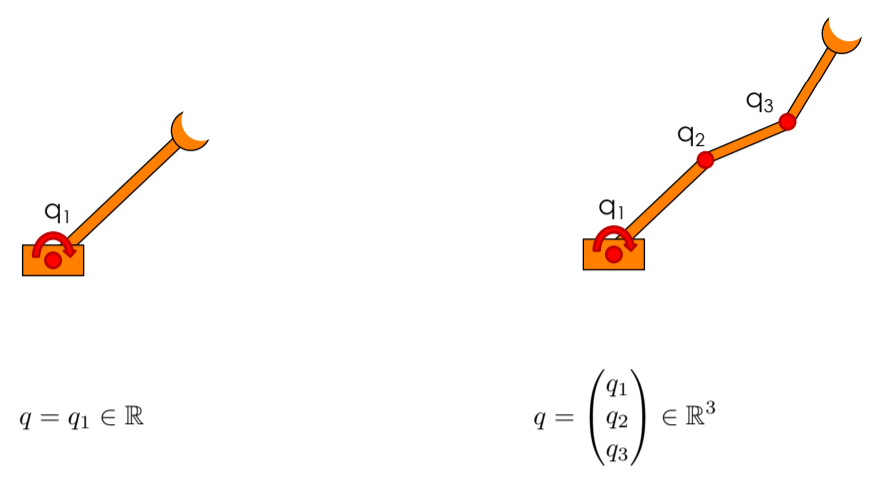
\includegraphics[width=0.9\linewidth]{imgs/joint_space_example.png}
  \caption{Example of joint space: one-joint system with $q_1 \in \mathbb{R}$ (left), and a three-joint system with $q \in \mathbb{R}^3$ (right).}
\end{figure}

\hfill

\subsection{Mobile Robots}

In mobile robots, the control system is integrated directly into the robot. These systems can also receive inputs from external devices, such as a remote control unit.

\subsubsection*{Wheeled Mobile Robots}

Wheels are considered the most appropriate solution for many mobile robot applications. A configuration with three wheels is sufficient to guarantee static stability. The number and type of wheels, as well as their arrangement, depend on the specific application requirements. In this course, the focus will be on Wheeled Mobile Robots (WMR), since they are the most widely used type of industrial mobile robots.

\subsubsection*{Types of wheels}

Wheeled mobile robots can be equipped with different types of wheels, each offering different motion capabilities:

\begin{itemize}
  \item \textbf{Fixed wheel}: allows rolling motion along its axis but not rotation about the vertical axis.
  \item \textbf{Adjustable centered wheel}: similar to a caster but mounted with the pivot axis centered on the wheel; it can rotate about the vertical axis.
  \item \textbf{Castor wheel}: an unpowered wheel that can swivel, commonly used for passive support.
  \item \textbf{Omnidirectional wheel}: equipped with rollers mounted around its circumference, it allows motion in any direction on the plane.
\end{itemize}

\begin{figure}[H]
  \centering
  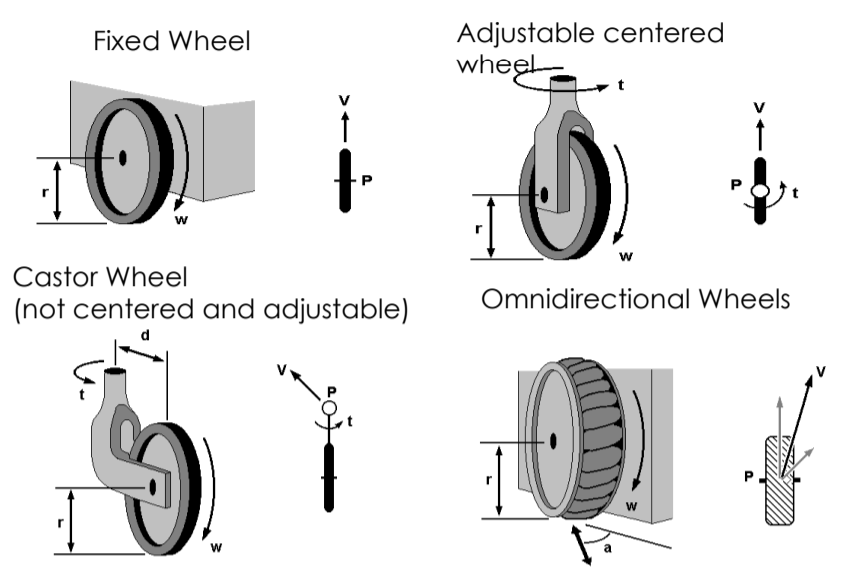
\includegraphics[width=0.9\linewidth]{imgs/types_of_wheels.png}
  \caption{Different types of wheels: fixed, adjustable centered, castor, and omnidirectional.}
\end{figure}

\subsubsection*{Omnidirectional Wheels}

Omnidirectional wheels exploit friction in a controlled manner to generate a transversal component of motion. This allows the robot to move laterally without changing its orientation.

These wheels are equipped with small rollers mounted around the circumference, which rotate independently and enable smooth sideways movement.

\begin{figure}[H]
  \centering
  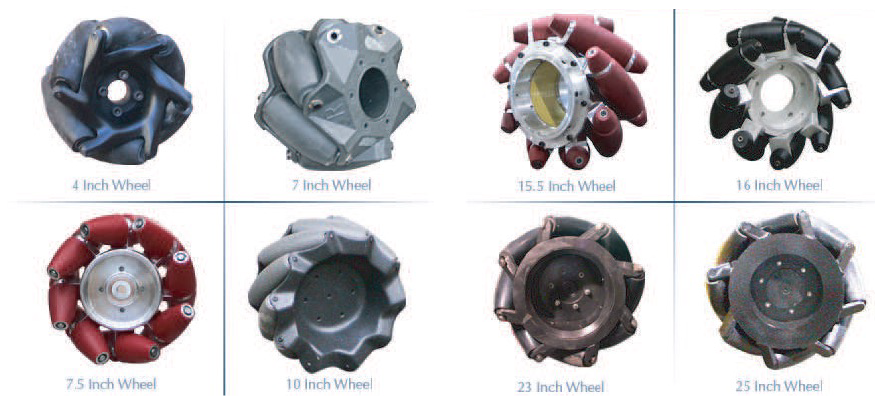
\includegraphics[width=\linewidth]{imgs/omnidirectional_wheels.png}
  \caption{Examples of omnidirectional wheels and their application in mobile robots.}
\end{figure}

\subsubsection*{Most Common Mechanical Structures}

\paragraph{Differential Drive} \hfill

The \textbf{differential drive} is one of the most common configurations for wheeled mobile robots. It consists of two independently actuated coaxial fixed wheels, which are used for both driving and steering.

To ensure static equilibrium, a third passive \textbf{castor wheel}—usually smaller than the actuated ones—is added.

Let $\omega_R$ and $\omega_L$ be the angular velocities of the right and left wheels respectively:
\begin{itemize}
  \item If $\omega_R = \omega_L$, the robot translates straight.
  \item If $\omega_R = -\omega_L$, the robot rotates in place.
  \item Intermediate values result in a general motion called \textbf{rototranslation}.
\end{itemize}

\begin{figure}[H]
  \centering
  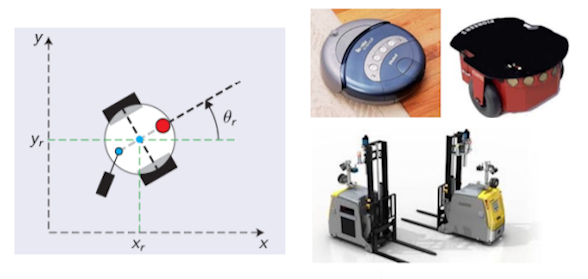
\includegraphics[width=0.8\linewidth]{imgs/differential_drive.png}
  \caption{Differential drive: top-view diagram and examples of real robots using this configuration.}
\end{figure}

Another common set of mechanical structures for wheeled mobile robots includes the \textbf{tricycle} and \textbf{car-like} configurations.

\paragraph{Tricycle} \hfill

This structure has two fixed back wheels and one steering front wheel. It can be either front- or rear-wheel driven.

\begin{itemize}
  \item \textbf{Pro:} High payload capacity.
  \item \textbf{Con:} Limited agility in maneuvering.
\end{itemize}

\paragraph{Car-like} \hfill

It has two fixed and aligned rear wheels and two steering, aligned front wheels. It can also be either front- or rear-wheel driven.

\begin{itemize}
  \item \textbf{Pro:} High payload capacity.
  \item \textbf{Con:} Limited agility in maneuvering.
\end{itemize}

\begin{figure}[H]
  \centering
  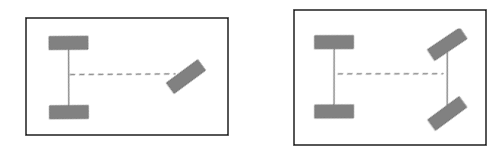
\includegraphics[width=0.85\linewidth]{imgs/tricycle_car_like.png}
  \caption{Mechanical structures: tricycle configuration (left) and car-like configuration (right).}
\end{figure}

\hfill

\subsection{Configuration Space}

The \textbf{configuration} of a robot is a complete specification of the position of every point of the robot.

The set of all possible configurations forms an $n$-dimensional space called the \textbf{configuration space} or \textbf{C-space}.

Each configuration corresponds to a single point in the configuration space.

Since the robot is composed of rigid bodies of known shape, only a limited number of \textbf{configuration parameters} are required to fully define the configuration.

\begin{figure}[H]
  \centering
  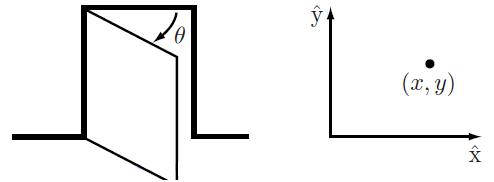
\includegraphics[width=0.55\linewidth]{imgs/configuration_space.png}
  \caption{Examples of configuration representation: position $(x, y)$ and orientation $\theta$.}
\end{figure}

For \textbf{robotic arms}, the configuration parameters are the joint variables $q_i$. In this case, the configuration space coincides with the \textbf{joint space}, represented as:
\[
q = 
\begin{pmatrix}
q_1 \\
\vdots \\
q_n
\end{pmatrix}
\in \mathbb{R}^n
\]

For \textbf{mobile robots}, the configuration parameters must describe the position and orientation of all relevant moving parts. For example:
\begin{itemize}
  \item A differential-drive robot may be described by $q = [x_r, y_r, \theta_r]^T \in \mathbb{R}^3$;
  \item A more complex mobile robot may require $q = [x_r, y_r, \theta_r, \phi_r]^T \in \mathbb{R}^4$.
\end{itemize}

In both cases, the configuration space (\textbf{C-space}) is the set of all possible configurations that the robot can assume.

\begin{figure}[H]
  \centering
  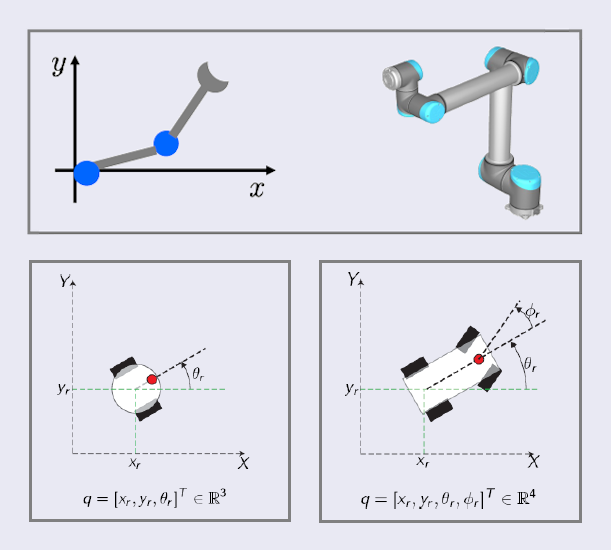
\includegraphics[width=0.9\linewidth]{imgs/configuration_space_examples.png}
  \caption{Configuration space for a robotic arm (top) and mobile robots (bottom left: $\mathbb{R}^3$, bottom right: $\mathbb{R}^4$).}
\end{figure}

\hfill

\subsection{Take-home Message}

Robotic arms and wheeled mobile robots are the most widely used robotic systems in industrial applications.

The most common mechanical configurations for robotic arms are the \textbf{cartesian} and the \textbf{anthropomorphic} ones.

For wheeled mobile robots, the most frequent configurations include the \textbf{differential drive}, the \textbf{tricycle}, and the \textbf{car-like} setups.

Finally, the \textbf{configuration parameters} of a robot define the position of all its parts. For robotic arms, the configuration space (\textbf{C-space}) corresponds to the joint space.

\newpage
\section{Robot Kinematics and Dynamics}

\subsection{Locate the robot and the objects in the scene}

This subsection introduces the fundamental question in robot kinematics: how to describe the relative positions and orientations of objects in a robotic environment. In particular, it requires determining the spatial relationships between different elements in the scene, such as the robot arm, its base, the mobile platform, the conveyor belt, and surrounding boxes.

The key questions are:

\begin{itemize}
  \item Where is the tool with respect to the base of the robot arm?
  \item Where is the mobile robot with respect to the arm base?
  \item Where is the box with respect to the mobile robot?
  \item Where is the conveyor belt with respect to the robot?
\end{itemize}

These questions are essential for defining the \textbf{coordinate frames} of each object and for understanding \textbf{how to transform} positions and orientations from one frame to another using homogeneous transformations. This is a prerequisite for solving forward and inverse kinematics problems, motion planning, and control.

\hfill

\subsection{Where is the part of interest of the robot?}

The primary kinematic problem in robotics is \textbf{how to describe the position and orientation of a robot component, such as an end-effector or a mobile base, with respect to a desired reference frame}.

This is essential because robot control, planning, and coordination rely on being able to mathematically describe “where” a certain component of the robot is located.

\textbf{Kinematics of the robot} is therefore:
\begin{itemize}
  \item fundamental for understanding how to use a robot;
  \item a problem that needs a clear and sound mathematical formalization.
\end{itemize}

The solution to this problem relies on the use of \textbf{reference frames}, often attached to relevant parts of the robot or to the environment. The \textbf{Body Frame} is the coordinate system fixed to the robot itself (e.g., at the base of a mobile platform or at a specific link of a manipulator). It moves with the robot and is used to express its configuration.

The diagram illustrates this idea: the robot's body frame (local frame) is shown inside a global reference frame (e.g., the room or map). The position and orientation of the body frame with respect to the global frame define the robot's pose.

\begin{figure}[H]
  \centering
  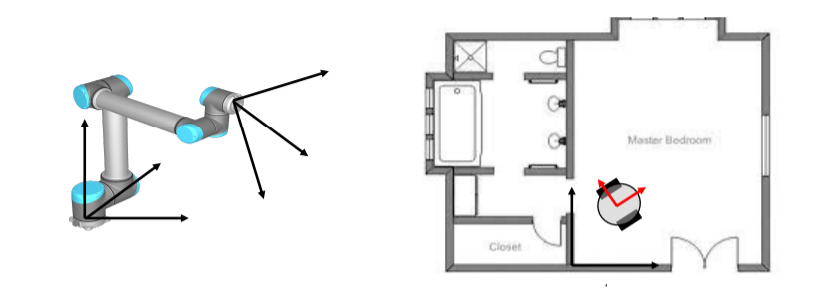
\includegraphics[width=\linewidth]{imgs/part_of_interest_kinematics.png}
  \caption{The robot’s body frame in a global environment frame.}
\end{figure}

\hfill

\subsection{Rigid Body Kinematics}

To analyze and control a robot, we must understand the kinematics of its components. Since a robot is composed of a sequence of rigid bodies (e.g., links in a manipulator), we must study the motion of rigid bodies to address robot kinematics properly.

\textbf{Key concepts:} a robot is made up of one or more rigid bodies connected by joints; understanding robot kinematics therefore requires first understanding \textbf{rigid body kinematics} and the mathematical tools developed for rigid body motion, such as coordinate transformations and rotation matrices.

The central question remains the same: \textit{"How can we describe the position and orientation of a rigid body with respect to a desired reference frame?"} This question is foundational and guides the development of the entire kinematic model of the robot.

To describe the position of objects in space, we use an \textbf{orthonormal reference frame} $F$, composed of three mutually orthogonal unit vectors (versors) $\hat{x}, \hat{y}, \hat{z}$, which define the orientation of the axes and intersect at an origin $O$.

\begin{itemize}
  \item Each versor defines the direction of an axis:
    \[
    \hat{x} = \begin{pmatrix}1 \\ 0 \\ 0\end{pmatrix}, \quad
    \hat{y} = \begin{pmatrix}0 \\ 1 \\ 0\end{pmatrix}, \quad
    \hat{z} = \begin{pmatrix}0 \\ 0 \\ 1\end{pmatrix}
    \]
  \item These versors form the basis of the frame $F$.
  \item A point $P$ in space can be located with respect to the frame $F$ using its coordinates $(x_P, y_P, z_P)$, and expressed as:
    \[
    \vec{OP} = x_P \hat{x} + y_P \hat{y} + z_P \hat{z}
    \]
    or in vector form:
    \[
    \vec{OP} = 
    \begin{pmatrix}
    x_P \\
    y_P \\
    z_P
    \end{pmatrix}
    \]
\end{itemize}

This formulation is the foundation for describing positions and motions in robotics, where the robot and its components are modeled as rigid bodies referenced to such frames.

\begin{figure}[H]
  \centering
  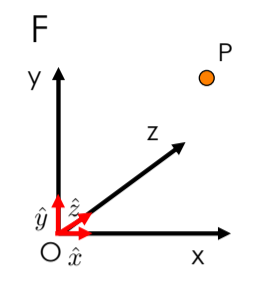
\includegraphics[width=0.3\linewidth]{imgs/rigid_body_reference_frame.png}
  \caption{Orthonormal reference frame $F$ and position vector of point $P$.}
\end{figure}

\hfill

\paragraph{Multiple Frames} \hfill

In robotic systems, it is common to use multiple coordinate frames to describe the positions of objects or parts of the robot. Each frame may be attached to a different body or component (e.g., base, end-effector, sensor).

\begin{itemize}
  \item Let $F_1$ and $F_2$ be two different reference frames.
  \item A point $P$ in space can be represented in both frames:
    \begin{itemize}
      \item $^1P$: coordinates of $P$ expressed in frame $F_1$.
      \item $^2P$: coordinates of $P$ expressed in frame $F_2$.
    \end{itemize}
  \item \textbf{In general,} the coordinate vectors $^1P$ and $^2P$ are different, because they are expressed with respect to different axes and origins.
\end{itemize}

To convert between representations in different frames, we use \textbf{coordinate transformations}, typically involving rotation and translation operations.

\begin{figure}[H]
  \centering
  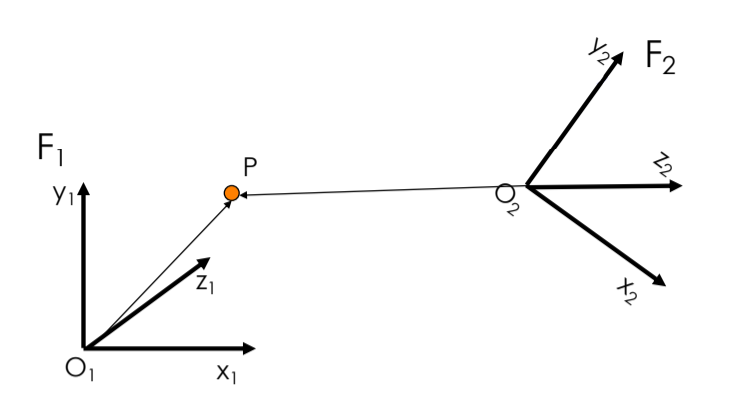
\includegraphics[width=0.65\linewidth]{imgs/multiple_frames.png}
  \caption{A point $P$ described in two different reference frames: $F_1$ and $F_2$.}
\end{figure}

\hfill

\paragraph{Pose and Body Frame} \hfill

A \textbf{rigid body} is defined as an object made up of a set of points that maintain a constant relative position. This implies that the body does not deform.

To describe a rigid body in space, we define its \textbf{pose}, which includes:
\begin{itemize}
  \item \textbf{Position}: the location of a point (usually the origin of the body frame) in a reference frame.
  \item \textbf{Orientation}: the angular configuration of the body frame with respect to the reference frame.
\end{itemize}

The pose of a rigid body is fully described by the pose of a frame rigidly attached to it, called the \textbf{body frame} ($F_B$).

\begin{itemize}
  \item The body frame moves with the rigid body.
  \item Its origin $O_B$ and axes $(x_B, y_B, z_B)$ define the configuration of the rigid body.
  \item The pose of the rigid body is defined with respect to a fixed reference frame, such as $F_0$.
\end{itemize}

\begin{figure}[H]
  \centering
  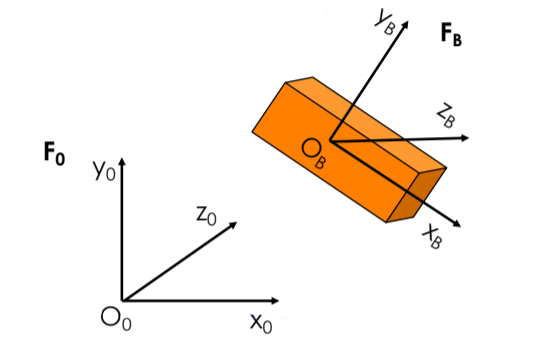
\includegraphics[width=0.6\linewidth]{imgs/pose_body_frame.png}
  \caption{Pose of a rigid body defined by the position and orientation of its body frame $F_B$ with respect to the reference frame $F_0$.}
\end{figure}

\hfill

\paragraph{Relative Position} \hfill

The \textbf{position} of a rigid body $B$ with respect to a fixed reference frame $F_0$ is defined by the position of the origin $O_B$ of the body frame $F_B$ relative to the origin $O_0$ of $F_0$.

\begin{itemize}
  \item This position is represented by the vector ${}^0\mathbf{O}_B$, which gives the coordinates of $O_B$ in frame $F_0$.
  \item It is written as:
    \[
    {}^0\mathbf{O}_B = 
    \begin{pmatrix}
      {}^0 O_{Bx} \\
      {}^0 O_{By} \\
      {}^0 O_{Bz}
    \end{pmatrix}
    =
    {}^0 O_{Bx} \hat{x}_0 + {}^0 O_{By} \hat{y}_0 + {}^0 O_{Bz} \hat{z}_0
    \]
  \item This vector describes the \textbf{relative position} of the body frame $F_B$ in the fixed frame $F_0$.
\end{itemize}

\begin{figure}[H]
  \centering
  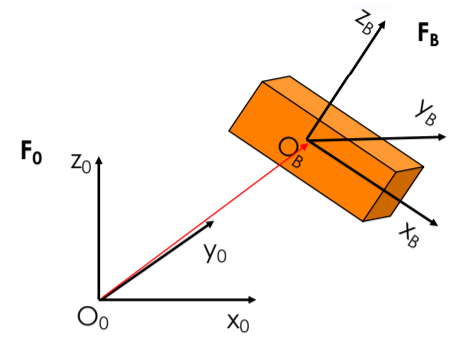
\includegraphics[width=0.5\linewidth]{imgs/relative_position.png}
  \caption{Relative position of the body frame $F_B$ with respect to the fixed frame $F_0$.}
\end{figure}

\hfill

\paragraph{Relative Orientation} \hfill

The orientation of a rigid body frame $F_B$ with respect to a reference frame $F_0$ can be described using different mathematical tools. The most common are:

\textbf{Rotation Matrix}: the orientation of $F_B$ with respect to $F_0$ is given by the rotation matrix ${}^0R_B \in SO(3)$; the inverse orientation (from $F_0$ to $F_B$) is given by the transpose
\[
{}^B R_0 = ({}^0 R_B)^T
\]
and rotation matrices compose via matrix multiplication,
\[
R_{AC} = R_{AB} \cdot R_{BC}.
\]

\textbf{Euler Angles}: orientation can also be represented by three sequential angles $(\rho, \vartheta, \varphi)$ describing rotations around selected axes (e.g., ZYX or XYZ convention), a formulation that is intuitive but affected by singularities (gimbal lock).

\textbf{Unit Quaternions}: a compact and non-singular representation of orientation, useful for interpolation (e.g., SLERP) and for avoiding gimbal lock. Quaternions use a four-element vector and compose through quaternion algebra.

\begin{figure}[H]
  \centering
  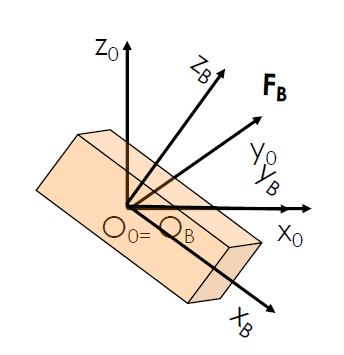
\includegraphics[width=0.4\linewidth]{imgs/relative_orientation.png}
  \caption{Orientation of frame $F_B$ with respect to $F_0$: axes are rotated but origins coincide.}
\end{figure}

\hfill

\paragraph{Homogeneous Transformations} \hfill

The \textbf{pose} of a rigid body with respect to a reference frame $F_0$ is defined by the pose of a frame $F_B$ rigidly attached to the body.

This pose is determined by two components: the \textbf{position}, i.e., the translation of the origin $O_B$ of frame $F_B$ with respect to the origin $O_0$ of the reference frame $F_0$ and expressed by the vector ${}^0\mathbf{O}_B$, and the \textbf{orientation}, namely the rotation of frame $F_B$ with respect to $F_0$, represented by the rotation matrix ${}^0R_B$.

Together, these two elements fully define the pose of the rigid body and can be compactly expressed using a \textbf{homogeneous transformation matrix} — which will be introduced and detailed in the following slides.

\begin{figure}[H]
  \centering
  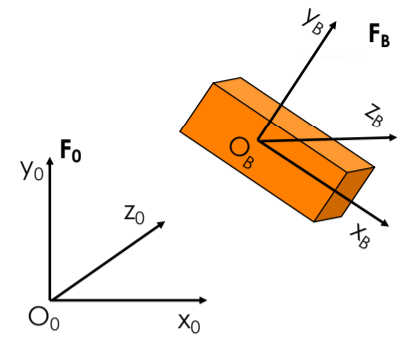
\includegraphics[width=0.4\linewidth]{imgs/homogeneous_transformations.png}
  \caption{The pose of the body frame $F_B$ with respect to the reference frame $F_0$ includes both translation and rotation.}
\end{figure}

To express both the position and orientation of a frame $F_1$ with respect to another frame $F_0$, we introduce the concept of a \textbf{homogeneous transformation}.

Consider a point $P$ expressed in frame $F_1$. Its coordinates in frame $F_0$ are given by:
\[
{}^0\!p = {}^0\!O_1 + {}^0\!R_1\, {}^1\!p
\]
This combines a translation (${ }^0\!O_1$) and a rotation (${ }^0\!R_1$). To make this operation more compact and composable, we adopt \textbf{homogeneous coordinates}.

\textbf{Homogeneous coordinates:}
\[
\tilde{p} = 
\begin{pmatrix}
p \\
1
\end{pmatrix}
\quad \text{(4x1 vector)}
\]

\textbf{Homogeneous transformation matrix:}
\[
{}^0\!T_1 =
\begin{pmatrix}
{}^0\!R_1 & {}^0\!O_1 \\
\mathbf{0} & 1
\end{pmatrix}
\quad \text{(4x4 matrix)}
\]

\textbf{Transformation of a point:}
\[
{}^0\!\tilde{p} = {}^0\!T_1\, {}^1\!\tilde{p}
\]

This matrix $T \in SE(3)$ (Special Euclidean group) allows us to perform roto-translations using a single matrix multiplication. The last row is always $\begin{pmatrix} 0 & 0 & 0 & 1 \end{pmatrix}$.

\begin{figure}[H]
  \centering
  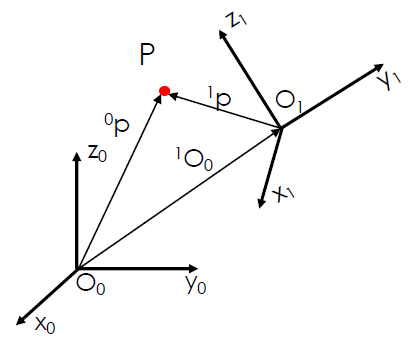
\includegraphics[width=0.5\linewidth]{imgs/homogeneous_point_position.png}
  \caption{Homogeneous transformation of a point $\tilde{p}$ from frame $F_1$ to frame $F_0$.}
\end{figure}

\textbf{Invertibility:}
The transformation matrix is always invertible. Its inverse is:
\[
{}^1\!T_0 =
\begin{pmatrix}
{}^1\!R_0 & -{}^1\!R_0\,{}^0\!O_1 \\
\mathbf{0} & 1
\end{pmatrix}
\]

This allows us to compute the pose of $F_0$ with respect to $F_1$ if the opposite is known.

\textbf{Composition of Transformations:}
Homogeneous transformations can be composed:
\[
{}^0\!T_2 = {}^0\!T_1\, {}^1\!T_2
\]
\[
{}^0\!\tilde{p} = {}^0\!T_2\, {}^2\!\tilde{p} = {}^0\!T_1\, {}^1\!T_2\, {}^2\!\tilde{p}
\]

This means that chains of transformations can be applied through successive matrix multiplications.

\begin{figure}[H]
  \centering
  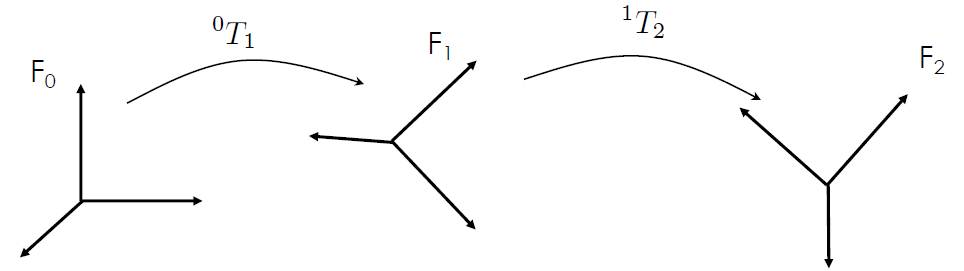
\includegraphics[width=\linewidth]{imgs/homogeneous_chain_composition.png}
  \caption{Composing transformations between multiple frames: $F_0 \rightarrow F_1 \rightarrow F_2$.}
\end{figure}

\hfill

\subsection{Homogeneous Transformations in Robotics}

Homogeneous transformations are widely used in robotics to describe the pose of robots and objects with respect to:
\begin{itemize}
  \item a fixed reference frame;
  \item neighboring or connected frames.
\end{itemize}

For example, consider a set of mobile robots each associated with a local frame $F_i$. Their pose with respect to a global frame $F_0$ is expressed by ${}^0T_i$, while their relative pose with respect to neighbors is expressed by transformations like ${}^1T_2$ or ${}^1T_3$.

\begin{figure}[H]
  \centering
  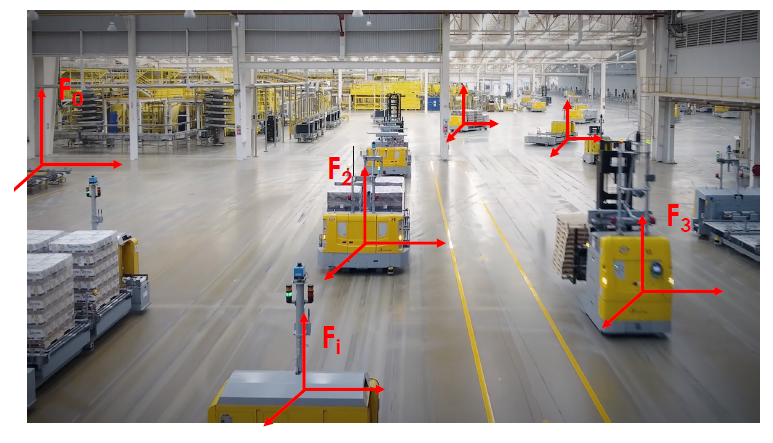
\includegraphics[width=0.75\linewidth]{imgs/homogeneous_robots_scene.png}
  \caption{Homogeneous transformations for multiple mobile robots.}
\end{figure}

The pose of the robot depends on the \textbf{configuration variables}, such as position $(x, y)$ and orientation $\vartheta$, and thus the homogeneous transformation matrix is:
\[
{}^0T_1 = \begin{pmatrix}
\cos\vartheta & -\sin\vartheta & 0 & x \\
\sin\vartheta & \cos\vartheta  & 0 & y \\
0 & 0 & 1 & 0 \\
0 & 0 & 0 & 1
\end{pmatrix}
\]

\begin{figure}[H]
  \centering
  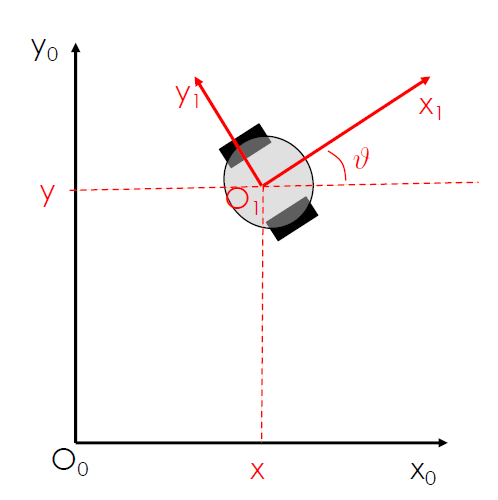
\includegraphics[width=0.45\linewidth]{imgs/homogeneous_planar_robot.png}
  \caption{Planar transformation of a wheeled mobile robot.}
\end{figure}

\paragraph{Planar robots:}
For wheeled mobile robots that move on a plane, the third row and third column of the matrix are always constant. Hence, we often reduce the transformation to a planar case:
\[
{}^0T_1 = \begin{pmatrix}
\cos\vartheta & -\sin\vartheta & x \\
\sin\vartheta & \cos\vartheta & y \\
0 & 0 & 1
\end{pmatrix}
\quad\text{with } {}^0R_1 \in SO(2), \quad {}^0O_1 \in \mathbb{R}^2
\]

\paragraph{Application in workspace:}
Homogeneous transformations are essential to relate different components of a robotic system:
\begin{itemize}
  \item ${}^0T_h$: hand with respect to robot base
  \item ${}^hT_{ob}$: object with respect to the hand
  \item ${}^0T_c$: camera with respect to the base
\end{itemize}

Using these matrices, one can map positions between components. For example, to express a point $p$ observed by a camera in the robot base frame:
\[
{}^0p = {}^0T_c \cdot {}^c p \qquad \forall p
\]

\begin{figure}[H]
  \centering
  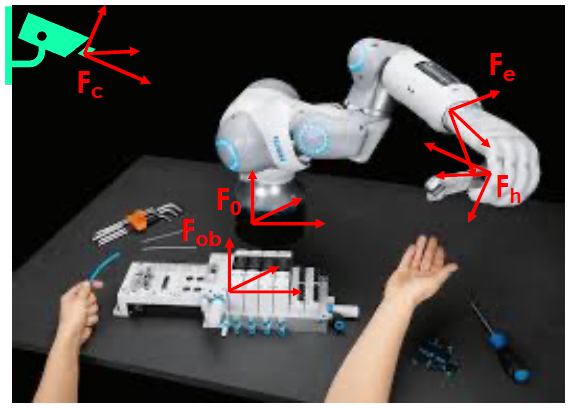
\includegraphics[width=0.65\linewidth]{imgs/homogeneous_workspace_robot.png}
  \caption{Frame transformations in a manipulation scenario (camera, robot, hand, object).}
\end{figure}

\hfill

\subsection{Homogeneous Transformations for Manipulators}

In the case of robotic manipulators, the pose of the end-effector (frame $F_n$) with respect to the robot base (frame $F_0$) depends on the configuration of the robot, specifically the values of the joint variables.

\paragraph{Direct (or Forward) Kinematics:}
It is the problem of determining the pose (position and orientation) of the end-effector given the joint variables. In other words, it computes the homogeneous transformation from base to end-effector:
\[
{}^0T_n = f(q_1, q_2, \dots, q_n)
\]
where $q_i$ are the joint variables (angles or displacements).

This is one of the \textbf{fundamental problems of robotics} and serves as the basis for motion planning, control, and simulation of robotic arms.

\begin{figure}[H]
  \centering
  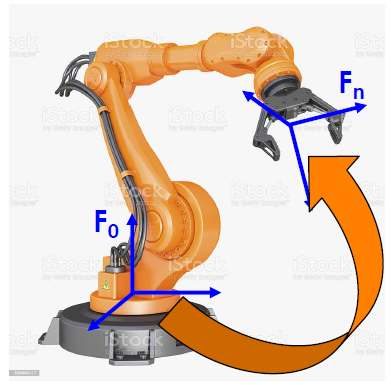
\includegraphics[width=0.4\linewidth]{imgs/forward_kinematics_robot_arm.png}
  \caption{Pose of the end-effector $F_n$ with respect to the robot base $F_0$, dependent on joint variables.}
\end{figure}

\hfill

\subsection{Forward Kinematics}

\paragraph{Definition:}
Forward kinematics (FK) consists in computing the pose of the end-effector of a manipulator given its configuration, i.e., the values of its joint variables. For an $n$-DOF robotic arm, this means:
\[
q \in \mathbb{R}^n \quad \Rightarrow \quad {}^0T_e(q) =
\begin{pmatrix}
{}^0R_e(q) & {}^0p_e(q) \\
\mathbf{0} & 1
\end{pmatrix}
\]

\paragraph{Key points:}
\begin{itemize}
  \item It allows to relate the joint variables (controlled inputs) to the pose of the end-effector (the part that interacts with the environment).
  \item It is crucial for understanding the movement of the end-effector resulting from joint actuation.
  \item It maps the \textbf{joint space} into the \textbf{task space}.
  \item The problem is \textbf{always solvable}, i.e., a unique pose can always be computed for a given configuration.
\end{itemize}

\paragraph{Solution method:}
Forward kinematics can be computed easily using the \textbf{Denavit-Hartenberg convention}, which systematically defines frame transformations along the links of a serial manipulator.

\hfill

\subsection{Inverse Kinematics}

\paragraph{Definition:}
Inverse kinematics (IK) is the problem of determining the joint configuration $q$ that produces a desired pose of the end-effector. Given:
\[
{}^0T_e = 
\begin{pmatrix}
{}^0R_e & {}^0p_e \\
\mathbf{0} & 1
\end{pmatrix}
\quad \Rightarrow \quad q = \text{IKINE}({}^0T_e)
\]

\paragraph{Importance:}
\begin{itemize}
  \item It is essential for converting motion specifications from the task space (e.g., Cartesian movements) into joint space commands that can be actuated by the robot.
  \item While forward kinematics is a direct computation, IK is often more challenging due to its mathematical structure.
\end{itemize}

\begin{figure}[H]
  \centering
  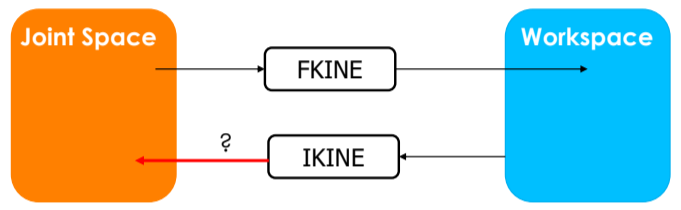
\includegraphics[width=0.6\linewidth]{imgs/ikine_mapping.png}
  \caption{Inverse kinematics maps the workspace pose back into the joint configuration space.}
\end{figure}

\paragraph{Challenges of Inverse Kinematics:}
\begin{itemize}
  \item IK equations are generally nonlinear.
  \item A closed-form solution may not always exist.
  \item There may be multiple or even infinite solutions (e.g., in redundant robots).
  \item Sometimes, no solution is admissible due to physical or kinematic constraints.
\end{itemize}

\begin{figure}[H]
  \centering
  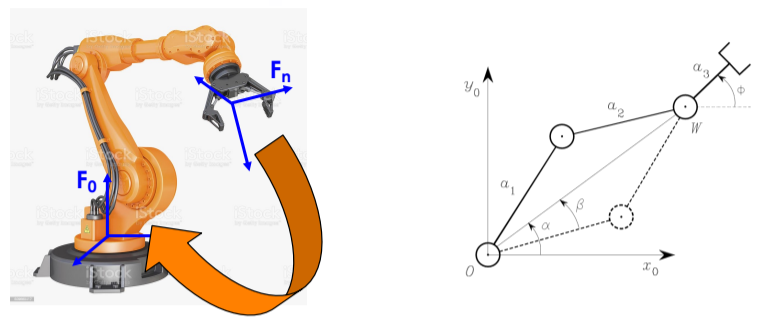
\includegraphics[width=0.8\linewidth]{imgs/ikine_robot_diagram.png}
  \caption{Example of a manipulator and schematic representation of link lengths and joint angles.}
\end{figure}

\paragraph{Solution Methods:}
\begin{itemize}
  \item \textbf{Closed-form}: Only possible in specific structures, usually using trigonometry or algebraic manipulation.
  \item \textbf{Numerical methods:} Needed when analytical solution is not feasible. Examples include:
  \begin{itemize}
    \item BFGS (Broyden-Fletcher-Goldfarb-Shannon)
    \item Levenberg–Marquardt
    \item Gradient projection methods
  \end{itemize}
  \item These methods minimize the error between the desired pose and the one obtained from the candidate solution.
\end{itemize}

\hfill

The direct and inverse kinematic problems are fundamental for describing the pose of the end-effector and the posture of the robot.

The composability of rotation matrices and of homogeneous transformation matrices is a very useful tool for representing the relative configurations between the robot(s) and other objects in the scene.

The Denavit–Hartenberg convention allows to have a standard for linking the joint configuration to the pose of the end-effector.

Inverse kinematics allows to map what happens in the workspace (e.g., specifications, desired poses), where no direct control is available, into the joint space, where it is possible to control the joints for achieving the desired behavior of the end-effector.

\hfill

Kinematics relates the configuration of the robot with the pose of the end-effector.

\begin{figure}[H]
    \centering
    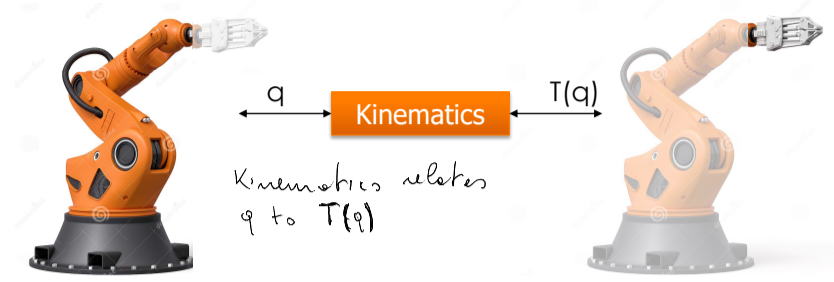
\includegraphics[width=1\linewidth]{imgs/differential_kinematics_begin.png}
\end{figure}

Kinematics relates the configuration of the robot in the joint space (determined by the joint variables) with the configuration of the end-effector in the workspace (determined, e.g., by homogeneous transformation matrix).

In order to map motions of the robot into motions of the end-effector and viceversa, it is important to relate velocities of the arm with velocities of the end-effector.

\hfill

\subsection{Differential Kinematics}

\paragraph{Def. 1:}

Consider a n-DOFs robotic arm. Given the speed of the joints, determine the linear and angular velocity of the end-effector.

It allows to map motions in the joint space into motions in the workspace.

It allows to understand how to move the joints in order to achieve a desired motion of the robot.

The relationship between joint velocities and the end-effector linear and angular velocity allows to characterize the mobility of the robot and to analyze its redundancy.

Given any representation of the pose of the end-effector (homogeneous matrix, etc.) with respect to a given frame (e.g., the base frame), the \textbf{velocity of the end-effector} can be represented by a 3-dimensional translational velocity and by a 3-dimensional angular velocity. \textit{Note:} This is called \textbf{Twist}.
  
The problem addressed by differential kinematics is to find a relation between the speed of the joints and the linear and angular velocity of the end-effector.

\textbf{Def. 2:} Consider a n-DOFs robotic arm, where $q = (q_1, \dots, q_n)^T$ is the joint vector. Express the linear and angular velocities of the end-effector $\dot{p}_e$ and $\omega_e$ as a function of the joint speed $\dot{q} = (\dot{q}_1, \dots, \dot{q}_n)^T$.

The sought relations are both linear in the joint velocities, which means:

\[
\dot{p}_e = J_P(q) \dot{q}
\]
\[
\omega_e = J_O(q) \dot{q}
\]

$\mathbf{J_P(q)}$: $(3 \times n)$ matrix relating the contribution of the joint velocities to the end-effector linear velocity $\dot{p}_e$.

$\mathbf{J_O(q)}$: $(3 \times n)$ matrix relating the contribution of the joint velocities to the end-effector angular velocity $\omega_e$.

In compact form, these relations can be written as:

\[
v_e = 
\begin{bmatrix}
\dot{p}_e \\
\omega_e
\end{bmatrix}
= J(q) \dot{q}
\quad\text{(6-dimensional vector)}
\]

This represents the manipulator \textbf{differential kinematics} equation, and the vector $v_e$ is called \textbf{generalized velocity} or \textbf{twist} of the end-effector.

The $6 \times n$ matrix $J(q)$ is the \textbf{geometric Jacobian} of the robot, where $n$ is the number of DOFs:
  \[
  J(q) = 
  \begin{pmatrix}
  J_P(q) \\
  J_O(q)
  \end{pmatrix}
  \]

In general, it depends on the joint variables.
  
It is possible to write:

\[
  J(q) =
  \begin{pmatrix}
  J_{P_1} & \dots & J_{P_n} \\
  J_{O_1} & \dots & J_{O_n}
  \end{pmatrix}
\]

whence:

\[
  J(q) \dot{q} =
  \begin{pmatrix}
  J_{P_1} \\
  J_{O_1}
  \end{pmatrix} \dot{q}_1 +
  \begin{pmatrix}
  J_{P_2} \\
  J_{O_2}
  \end{pmatrix} \dot{q}_2 + \dots +
  \begin{pmatrix}
  J_{P_n} \\
  J_{O_n}
  \end{pmatrix} \dot{q}_n
\]
  
\textit{Note (handwritten annotation):} In the case of two vectors, these sums indicate that we can move with velocities $\dot{q}_1$ and $\dot{q}_2$ along the directions defined by the respective vectors $\begin{pmatrix} J_{P_1} \\ J_{O_1} \end{pmatrix}$ and $\begin{pmatrix} J_{P_2} \\ J_{O_2} \end{pmatrix}$, i.e. on a plane.

The structure of each joint determines how the corresponding joint speed contributes to the twist.

\hfill

\paragraph{Kinematic Singularities} \hfill

The differential kinematics provides a linear relation between the twist of the end-effector $v_e$ and the joint velocities $\dot{q}$:
\[
v_e = J(q) \dot{q}
\]
\textit{Nota (annotazione a penna):} In pratica, la Jacobiana $J(q)$ ci dice quali movimenti può o non può eseguire il robot.

The configurations where $J(q)$ is \textbf{rank deficient} are termed \textbf{kinematic singularities}.
\textit{Nota (annotazione a penna):} Quando $J$ è rank-deficient, significa che manca il contributo di una colonna (perché è combinazione lineare di un'altra), ovvero alcune direzioni di movimento non possono essere raggiunte dal robot.

To find the singularities of a manipulator is of great interest for the following reasons:
\begin{itemize}
    \item Singularities represent configurations at which mobility of the structure is reduced, i.e., it is not possible to impose an arbitrary motion to the end-effector.
    \item When the structure is at a singularity, infinite solutions to the inverse kinematics problem may exist.
    \item In the neighbourhood of a singularity, small velocities in the operational space may cause large velocities in the joint space.
\end{itemize}

When the robot is in a singularity configuration, no value of joint velocities $\dot{q}$ exists for moving the end-effector in some direction.

\begin{figure}[H]
    \centering
    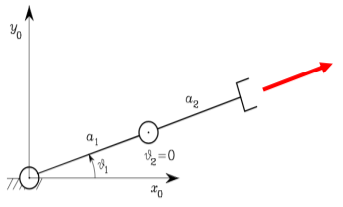
\includegraphics[width=0.6\linewidth]{imgs/kinematic_sing_1.png}
\end{figure}

If a robot has 6 DOFs, the Jacobian is square and the rank deficient configurations are those where:
\[
\det(J(q)) = 0
\]

Thus, all the kinematic singularities can be found by solving the algebraic equation $\det(J(q)) = 0$ in $q$.

\begin{itemize}
    \item The equation $\det(J(q)) = 0$ is very nonlinear and a numerical solver may be used for solving it.
\end{itemize}

They can be classified into:

\textbf{Boundary singularities:} occur when the manipulator is either out-stretched or retracted. They are easy to avoid by keeping the robot far from the boundary of its workspace.

\begin{figure}[H]
    \centering
    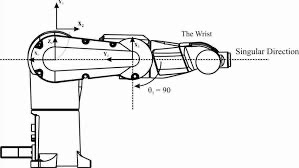
\includegraphics[width=0.6\linewidth]{imgs/boundary_singularity.png}
    \caption{Example of a boundary singularity when the manipulator is fully extended.}
\end{figure}

\textbf{Internal singularities:} occur inside the reachable workspace and are generally caused by the alignment of two or more axes of motion, or by the attainment of particular end-effector configurations. They are hard to avoid.

\begin{figure}[H]
    \centering
    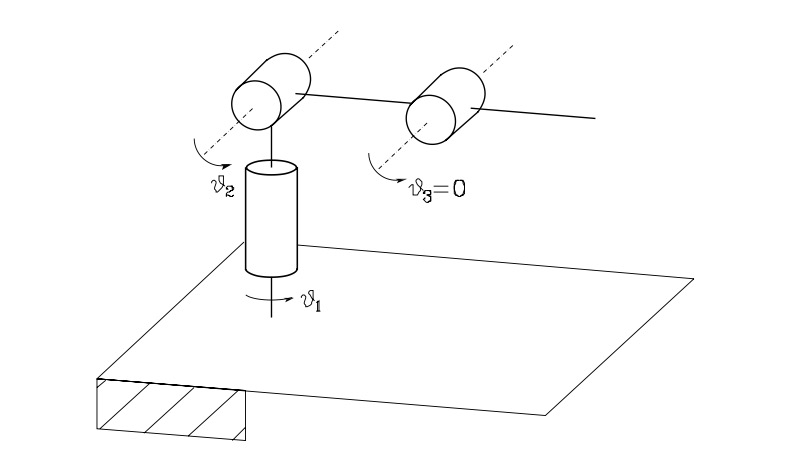
\includegraphics[width=0.6\linewidth]{imgs/internal_singularity.png}
    \caption{Example of an internal singularity due to axis alignment.}
\end{figure}

\hfill

\subsection{Inverse Differential Kinematics}

\textbf{Def.:} Consider a n-DOFs robotic arm, where $q = (q_1, \dots, q_n)^T$ is the joint vector. Given a desired twist $v_e$ for the end-effector, find the joint velocities that produce $v_e$.

This is a very important problem to be solved (often online) for finding the speed to control the joints for moving the end-effector with the desired twist $v_e$.

Thanks to the linear relation of the differential kinematics:

\[
    v_e = J(q) \dot{q}
\]

the inverse differential kinematics is much easier to address than inverse kinematics.

If $n = m$, i.e., the dimension of the joint space is the same as the one of the workspace, the Jacobian is square and the inverse differential kinematics problem can be solved by:

\[
    \dot{q} = J^{-1}(q) v_e
\]

If the Jacobian is \textbf{NOT} invertible, i.e., if $\det(J(q)) = 0$, the robot is in a singular configuration. Its mobility is limited and the inverse differential kinematics cannot be solved.

\textit{Nota (annotazione a penna):} Può accadere che la Jacobiana non sia invertibile perché essa non è una matrice costante, dato che dipende dalla configurazione degli angoli del robot.

It is necessary to plan the motion of the robot to keep it away from singular configurations. In this way, it is always possible to compute the motion of the joints to reproduce the desired motion of the end-effector.

If $n > m$, i.e., if the robot is redundant, the Jacobian is rectangular and the inverse does not exist.

If the Jacobian has full rank, then the inverse differential kinematics problem admits \textbf{infinitely many solutions}.

It is possible to exploit the concept of \textbf{pseudo-inverse of the Jacobian} for selecting a specific solution:

\[
\dot{q} = J^{+}(q) v_e
\quad\text{where}\quad
J^{+} = J^T (J J^T)^{-1}
\]

\textit{Nota (annotazione a penna):} $J^{+}$ is the pseudo-inverse.

In this case $\dot{q}$ is the minimum norm solution to the inverse differential kinematics problem. This means that:

\[
\|\dot{q}\| = \sqrt{\dot{q}_1^2 + \cdots + \dot{q}_n^2}
\]

is minimal, i.e. the pseudo inverse finds the lowest speed solution.

\textit{Nota (annotazione a penna):} Minore è la velocità, meglio è: minor sforzo sui motori e minor dispendio energetico.

\begin{figure}[H]
    \centering
    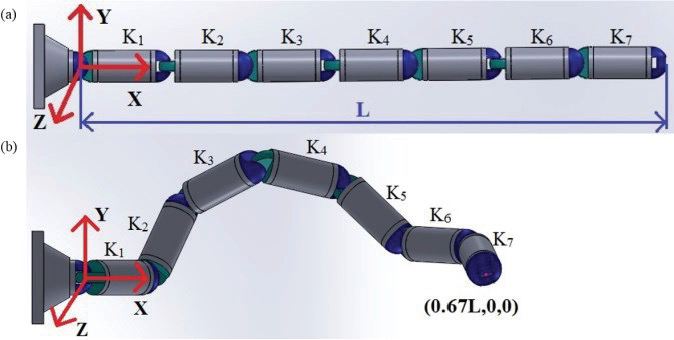
\includegraphics[width=1\linewidth]{imgs/inverse_diff_kine.png}
\end{figure}

Infinitely many joint speeds can instantaneously move the robot along a desired direction.

The pseudo inverse of the Jacobian exists only if the Jacobian is full rank. Thus, if the Jacobian is not full rank, the robot loses mobility and the inverse differential kinematics cannot be solved.

It is necessary to plan the motion of the robot to keep it away from singular configurations. In this way, it is always possible to compute the motion of the joints to reproduce the desired motion of the end-effector.

\textit{Nota (annotazione a penna):} Da una determinata velocità lineare posso ottenere la corrispondente velocità angolare:

\begin{figure}[H]
    \centering
    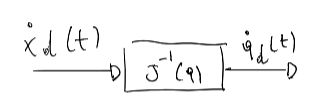
\includegraphics[width=0.4\linewidth]{imgs/inv_diff_kine_speeds.png}
\end{figure}

\[
J^{-1}(q) = \frac{1}{\det(J(q))} \, A^{T}
\]

$\det(J(q))$ is a continuous function.

\subsubsection*{Analytical Jacobian}

The Jacobian we saw before was geometric.

If the end-effector pose is specified in terms of a minimal number of parameters in the operational space, it is natural to compute the Jacobian via differentiation of the direct kinematics function with respect to the joint variables.

The translational velocity of the end-effector frame can be expressed as the time derivative of vector $\mathbf{p}_e$ representing the origin of the end-effector frame with respect to the base frame, i.e.,
    
\[
    \dot{\mathbf{p}}_e = \frac{\partial \mathbf{p}_e}{\partial \mathbf{q}} \dot{\mathbf{q}} = J_P(\mathbf{q}) \dot{\mathbf{q}}
\]

For what concerns the rotational velocity of the end-effector frame, the minimal representation of orientation in terms of three variables $\boldsymbol{\phi}_e$ can be considered. \textcolor{red}{Its time derivative in general differs from the angular velocity vector previously defined}.

\[
    \dot{\boldsymbol{\phi}}_e = \frac{\partial \boldsymbol{\phi}_e}{\partial \mathbf{q}} \dot{\mathbf{q}} = J_{\phi}(\mathbf{q}) \dot{\mathbf{q}}
\]

Upon these premises, the \textbf{differential kinematics equation} can be obtained as the time derivative of the direct kinematics equation, i.e.:

\[
\dot{x}_e =
\begin{bmatrix}
\dot{p}_e \\
\dot{\phi}_e
\end{bmatrix}
=
\begin{bmatrix}
J_P(q) \\
J_\phi(q)
\end{bmatrix}
\dot{q}
= J_A(q)\dot{q}
\]

where the \textbf{analytical Jacobian}

\[
J_A(q) = \frac{\partial k(q)}{\partial q}
\]

is different from the geometric Jacobian $J(q)$ since the end-effector angular velocity $\boldsymbol{\omega}_e$ with respect to the base frame is not given by $\dot{\phi}_e$.

It is possible to find the relationship between the angular velocity $\boldsymbol{\omega}_e$ and the rotational velocity $\dot{\phi}_e$ for a given set of orientation angles.

Equation relating the angular velocity to the time derivative of the Euler angles:

\[
\boldsymbol{\omega}_e = T(\phi_e)\dot{\phi}_e, \quad
T =
\begin{bmatrix}
0 & -\sin \varphi & \cos \varphi \, \sin \vartheta \\
0 & \cos \varphi & \sin \varphi \, \sin \vartheta \\
1 & 0 & \cos \vartheta
\end{bmatrix}.
\]

Once the transformation $T$ between $\boldsymbol{\omega}_e$ and $\dot{\phi}_e$ is given, the analytical Jacobian can be related to the geometric Jacobian as:

\[
\boldsymbol{v}_e =
\begin{bmatrix}
I & 0 \\
0 & T(\phi_e)
\end{bmatrix}
\dot{x}_e
= T_A(\phi_e)\dot{x}_e
\]

\[
J = T_A(\phi) J_A
\]

This relationship shows that $J$ and $J_A$, in general, differ.

The Analytical Jacobian is often used in control schemes. In fact, a minimal representation of the twist can be integrated for achieving the pose of the end-effector. This cannot be achieved using the geometric Jacobian since the integral of the angular velocity \textbf{is not} the orientation of the end-effector.

\[
\dot{q} \;\; \xrightarrow{\;\; J(q) \;\;} \;\; 
v_e = 
\begin{pmatrix}
\dot{p}_e \\ 
\omega_e
\end{pmatrix}
\;\; \xrightarrow{\;\; \int \;\;} \;\;
x_e = 
\begin{pmatrix}
p_e \\ 
\times
\end{pmatrix}
\quad \text{to control (wrong)}
\]

\begin{figure}[H]
    \centering
    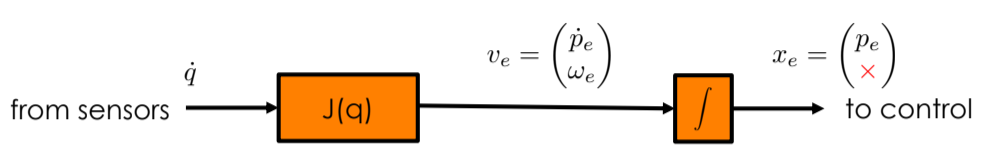
\includegraphics[width=0.85\linewidth]{imgs/diff_kine_1.png}
\end{figure}

\[
\dot{q} \;\; \xrightarrow{\;\; J_A(q) \;\;} \;\; 
v_e = 
\begin{pmatrix}
\dot{p}_e \\ 
\dot{\phi}_e
\end{pmatrix}
\;\; \xrightarrow{\;\; \int \;\;} \;\;
x_e = 
\begin{pmatrix}
p_e \\ 
\phi_e
\end{pmatrix}
\quad \text{to control (correct)}
\]

\begin{figure}[H]
    \centering
    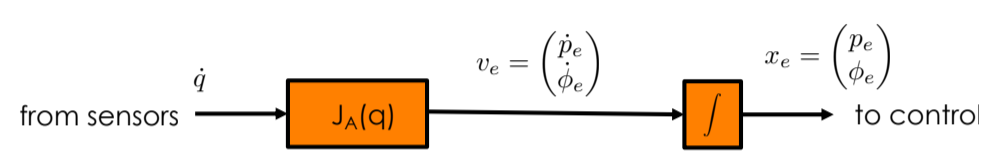
\includegraphics[width=0.85\linewidth]{imgs/diff_kine_2.png}
\end{figure}

\subsection{Statics}

\textbf{Def:} Consider a n-DOFs robotic arm. Given the force and the torque applied to the end-effector, determine the corresponding torques/forces applied to the joints.

It allows to map interactions in the workspace into actions on the joint space.

It allows to understand how to control the joints in order to achieve a desired interaction of the robot with the environment.

Let $\boldsymbol{\tau}$ denote the $(n \times 1)$ vector of joint torques/forces and $\boldsymbol{w}_e$ the $(6 \times 1)$ vector of generalized force, also called \textbf{wrench}, applied to the end-effector. 

The wrench has the following structure:

\[
\boldsymbol{w}_e =
\begin{pmatrix}
\boldsymbol{f}_e \\
\boldsymbol{\mu}_e
\end{pmatrix}, 
\qquad \boldsymbol{f}_e \in \mathbb{R}^3, \quad 
\boldsymbol{\mu}_e \in \mathbb{R}^3
\]

where $\boldsymbol{f}_e$ and $\boldsymbol{\mu}_e$ are the force and the torque applied to the end-effector.

The application of the \textit{principle of virtual work} allows the determination of the required relationship that can be summarized as:

\[
\boldsymbol{\tau} = J^T(q)\boldsymbol{w}_e
\]

stating that the relationship between the end-effector forces and the joint torques is established by the transpose of the manipulator geometric Jacobian.

\hfill

\subsection{Recap on Kinematics Relationship and Differential Kinematics}

\begin{figure}[H]
    \centering
    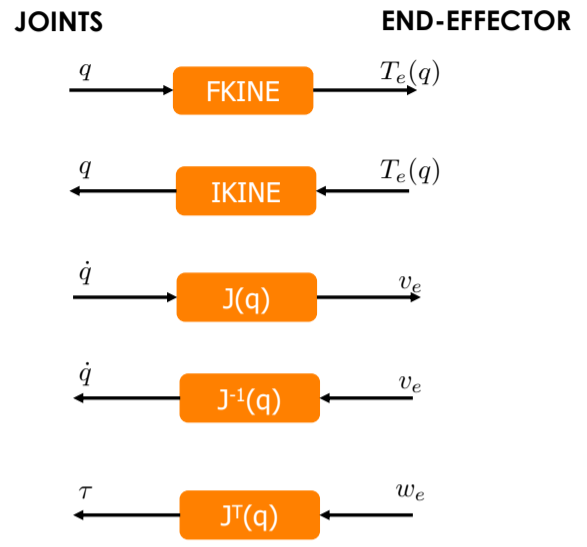
\includegraphics[width=0.65\linewidth]{imgs/kinematic_relationship.png}
    \caption{Kinematics Relationship}
\end{figure}

Differential kinematics and inverse differential kinematics are fundamental for mapping the motion of the robot into the motion of the end-effector and viceversa.
    
The Jacobian matrix is a fundamental object, describing the mobility of the end-effector.
    
Singularity configurations are points where the robot loses mobility in one or more directions.
    
The Jacobian allows to map wrenches applied to the end-effector into equivalent torques on the joints.

\hfill

Kinematics allows to capture the configuration of the robot and the pose of the end-effector.
    
In order to capture information about the behavior of the robot under the effect of external forces (e.g. gravity, wrenches on the end-effector, torques/forces on the joint), it is necessary to build a dynamic model of the manipulator.
    
The most common and useful strategy for building the dynamic model is the Euler-Lagrange formulation, that generalizes the second Newton law to multi-body systems.

\hfill

\subsection{Dynamics}

Joints can be actuated by linear forces (prismatic joints) or by torques (revolute joints).
    
The set of torques/linear forces is grouped in a vector $\tau \in \mathbb{R}^n$.

By applying a force/torque to the joints it is possible to change the configuration of the robot and, consequently, the pose of the end-effector.
    
Force/torques on the joints and external wrenches applied on the end-effector are the external action applied on the robot and that produce a motion of the overall structure.

\hfill

\subsection{Dynamic model in the joint space}

\textbf{Def:} Consider a n-DOFs robotic arm. Build the dynamic relation between the torques/forces acting on joints and the acceleration of the joints.

It allows to understand the effect of forces/torques on the joints on the motion of the robot.
    
It is the model that will be used for controlling the motion of the robot in the joint space.
    
The model can be built exploiting the Lagrangian formulation.

Using the Lagrangian formalism, the mechanics of the multi-body robotic arm leads to the following model:

\[
    M(q)\ddot{q} + C(q, \dot{q})\dot{q} + g(q) = \tau
\]

Joints can be affected by dynamic friction, due to the non-idealities in the coupling. Furthermore, an external wrench acting on the end-effector can produce extra torques acting on the robot. These effects can be modeled by adding external actions as:

\[
    M(q)\ddot{q} + C(q, \dot{q})\dot{q} + g(q) = \tau - D\dot{q} + J^T(q)w_e
\]

Usually the terms related to the physics of the robot are on the same side and the \textbf{Euler-Lagrange model in the joint space} is written as

\[
    M(q)\ddot{q} + C(q, \dot{q})\dot{q} + D\dot{q} + g(q) = \tau + J^T(q)w_e
\]

\hfill

\subsection{Properties of the Euler-Lagrange model}

$M(q)$ is a square, symmetric and positive definite matrix

\[
    M^T(q) = M(q), \qquad x^T M(q) x > 0 \quad \forall x \neq 0, \; x \in \mathbb{R}^n
\]  

This is the \textit{inertia}.

$D$ is a square, (usually) symmetric and positive definite matrix

\[
    D^T = D, \qquad x^T D x > 0 \quad \forall x \neq 0, \; x \in \mathbb{R}^n
\]  

This is the \textit{friction on all the joints}.  

The matrix $\dot{M}(q) - 2C(q,\dot{q})$ is \textbf{skew-symmetric} ($A^T = -A$)  

\[
    (\dot{M}(q) - 2C(q,\dot{q}))^T = -(\dot{M}(q) - 2C(q,\dot{q}))
\]  

\[
    x^T (\dot{M}(q) - 2C(q,\dot{q})) x = 0 \quad \forall x \neq 0, \; x \in \mathbb{R}^n
\]  

\hfill

To recap, the terms of the Euler--Lagrange model can be summarized as follows:

\begin{itemize}
    \item $\mathbf{M(q)}$: inertia matrix, square, symmetric and positive definite.
    \item $\mathbf{C(q,\dot{q})\dot{q}}$: Coriolis and centrifugal terms.
    \item $\mathbf{D\dot{q}}$: viscous friction and joint dissipative effects.
    \item $\mathbf{g(q)}$: gravity terms acting on the manipulator.
    \item $\mathbf{\tau}$: vector of joint torques/forces.
    \item $\mathbf{J^T(q)w_e}$: contribution of external forces (wrench) mapped to the joints through the Jacobian transpose.
\end{itemize}

\hfill

\subsection{Dynamic Model in the task space}

The dynamic model of the robot can be formulated also in the task space. This is useful for modeling the dynamic behavior of the end-effector.  

The dynamic model in the task space can be derived starting from the dynamic model in the joint space.  

The most common formulation of the dynamic model in the task space represents the pose of the end-effector as a $6 \times 1$ vector, using Euler angles for representing the pose.

The \textbf{dynamic model in the task space} is given by:
\[
    M_A(x_e)\ddot{x}_e + C_A(x_e, \dot{x}_e)\dot{x}_e + D_A\dot{x}_e + g_A(x_e) = w_d + w_f
\]

where:
\[
    M_A(x_e) = \left(J_A M^{-1} J_A^T \right)^{-1}
\]
\[
    C_A(x_e, \dot{x}_e)\dot{x}_e = J_A^{-T} C \dot{q} - M_A \dot{J}_A \dot{q}
\]
\[
    D_A = J_A^{-T} D
\]
\[
    g_A = J_A^{-T} g
\]

\hfill

The dynamic model in the task space enjoys the same properties as the dynamic model in the joint space.  

Unlike the dynamic model in the joint space, the dynamic model in the task space is well defined when the robot is not close to singularities.  

\newpage

\section{Control of Robotic Systems}

\subsection{Controlling a robot}

\textbf{Def.:} Determinate, using proper algorithms, the control inputs such that the robot behaves as desired both kinematically (position/velocity) and/or dynamically (forces, interaction).

Before designing the control algorithms, it is necessary to deal with important preliminary issues:

\begin{itemize}
    \item \textbf{Actuation:} What is the control input of the robot?
    \item \textbf{Architecture:} What is the structure of the control system for a robot?
    \item \textbf{Planning:} How to define and design the desired behavior of the robot?
    \item \textbf{Stability:} How to guarantee a robust behavior of the robot?
\end{itemize}

\hfill

\subsection{Actuation}

Every joint is actuated by a \textbf{servomotor}.
    
Several types of servomotors can be used:

\begin{itemize}
    \item Pneumatic/hydraulic actuators (very high payload)
    \begin{itemize}
        \item Low control flexibility
        \item Used for opening/closing tools, simple motions
        \item Very slow
    \end{itemize}
    \item \textbf{Electrical motors}
    \begin{itemize}
        \item High control flexibility
        \item Trajectory tracking
        \item No high payload
    \end{itemize}
\end{itemize}
    
The most used electrical servomotors are:

\begin{itemize}
    \item DC motors with permanent magnets
    \item Brushless motors
\end{itemize}

\textit{Remember that we control the motors to control the robot.}

\newpage

\subsubsection*{Servomotor}

\begin{wrapfigure}[21]{r}{0.32\linewidth} 
  % l’opzione [12] dice a LaTeX di riservare solo 12 righe di testo in altezza
  \vspace{-1.5\baselineskip}
  \centering
  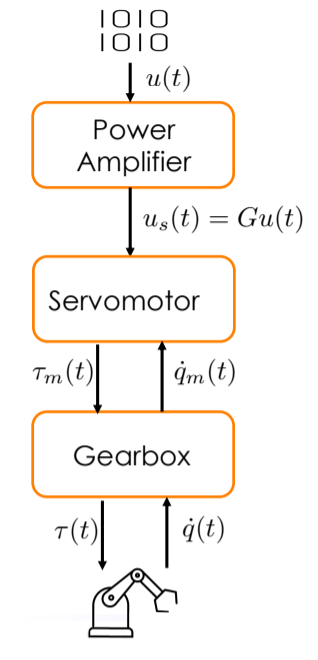
\includegraphics[width=\linewidth]{imgs/control_process_with_servomotors.png}
  \caption{Control process with servomotors.}
\end{wrapfigure}


The control process starts from digital information (data) given by the controller. 
This information $u(t)$ represents the \textbf{control signals}.

A \textbf{Power Amplifier} transforms them into a physical signal $u_s(t)=G\,u(t)$ to control the motor.

The \textbf{Servomotor} then produces movement described by angular velocity $\dot{q}_m(t)$ and torque $\tau_m(t)$.

This torque is transmitted through a \textbf{Gearbox}, which adapts speed and torque to the mechanical structure.

Finally, the robot joints experience the movement: angular velocity $\dot{q}(t)$ and torque $\tau(t)$, i.e. the \textbf{torque that moves the joints}.

\textit{Notes:}
\begin{itemize}
  \item The input comes as digital information from the controller.
  \item The servomotor generates torque and angular velocity.
  \item The gearbox ensures that the torque is adapted to effectively move the robot joints.
\end{itemize}

\hfill

\subsubsection*{DC Motors}

DC motors are \textbf{mainly designed for achieving high rotational speeds with low torques}.  
They are typically used in high-speed and high-volumes industrial automation.  

\textit{Note: In industrial applications, we want to move as fast as possible.}

The angular position/velocity of the rotating axis can be measured by sensors:
\begin{itemize}
    \item Position $\rightarrow$ encoder
    \item Velocity $\rightarrow$ encoder (+processing), resolver
    \item Torque/Current $\rightarrow$ torque sensor, current sensors
\end{itemize}

\textbf{Low-level position/velocity control is embedded} in servomotors.  

\textit{Note: The controller integrates the motor movement at the lowest input level.}

\hfill

\subsubsection*{Gearbox}

A \textbf{gearbox} is a mechanical device that is used to increase the output torque or change the speed of the motor.  

The motor shaft is connected to one end of the gearbox and, through the internal configuration of the gears of the gearbox, it provides an output torque and a specific speed determined by the gear ratio.  

\[
\begin{cases}
t(t) = k t_m(t) \\
\omega_m(t) = k \, \omega(t)
\end{cases}
\]

with $k > 0$ the \textbf{gain of the gearbox}.  

From the equations it follows that:
\[
t(t)\,\omega(t) = t_m(t)\,\omega_m(t)
\]
that is, \textbf{power is preserved}.  

\textit{Notes:}  
\begin{itemize}
    \item The input is the motor’s angular velocity $\omega_m$ and torque $t_m$.  
    \item The output is the angular velocity $\omega$ and torque $t$.  
    \item Increasing torque implies decreasing velocity: \textit{more torque, but less velocity}.  
    \item These relations allow us to exchange torque and velocity according to the gear ratio.  
    \item This transformation maintains power balance.  
    \item Intuitively: more power and force can be achieved at the expense of speed, and vice versa.  
\end{itemize}

\hfill

\subsubsection*{Servomotors}

The use of servomotors in robotics requires \textbf{high torques}, for moving the links connected to the joints, but \textbf{lower speeds} with respect to the ones required in standard industrial automation applications.  

Gearboxes are exploited for achieving the right balance between speed and torque of the joints.  

\[
\begin{cases}
\tau(t) = K \tau_m(t) \\
\dot{q}_m(t) = K \dot{q}(t)
\end{cases}
\quad
K = 
\begin{pmatrix}
K_1 & 0   & \dots & 0 \\
0   & K_2 & \dots & 0 \\
\vdots & \vdots & \ddots & \vdots \\
0   & 0   & \dots & K_n
\end{pmatrix}, 
\quad K_i \gg 1
\]

The torque of the motors is amplified and the speed is attenuated.  

\textit{Notes:}  
\begin{itemize}
    \item $\tau$ is the output torque at the joint, $\tau_m$ is the torque of the motor.  
    \item $\dot{q}$ is the angular velocity of the joint, $\dot{q}_m$ is the angular velocity of the motor.  
    \item Since $K_i \gg 1$, we obtain much larger torque at the output, but lower angular velocity.  
    \item Power is preserved:  
    \[
    \tau = K \tau_m, \quad \dot{q}_m = K \dot{q}, \quad \Rightarrow \quad \tau^T \dot{q} = \tau_m^T \dot{q}_m
    \]  
    \item Intuitively: the gearbox amplifies the torque and reduces the velocity while maintaining the power balance.  
\end{itemize}

\hfill

\subsection{Actuation and Mechanics}

What is directly controlled is the input of the servomotors.  

The dynamics of the servomotors and the gain of the gearboxes have a strong impact on the system to be controlled.  

\[
M(q)\ddot{q} + C(q,\dot{q})\dot{q} + D\dot{q} + g(q) = \tau
\quad \text{(Euler-Lagrange equation)}
\]

\[
\begin{cases}
\tau(t) = K \tau_m(t) \\
\dot{q}_m(t) = K \dot{q}(t)
\end{cases}
\quad
K = 
\begin{pmatrix}
K_1 & 0   & \dots & 0 \\
0   & K_2 & \dots & 0 \\
\vdots & \vdots & \ddots & \vdots \\
0   & 0   & \dots & K_n
\end{pmatrix}, 
\quad K_i \gg 1
\]

The driving torque of each motor is controlled.  

The driving torque of the actuator produces a torque on the robot joint \textit{through the gearbox}.

\hfill

Combining the mechanics of the robot and the gearbox constitutive equations:

\[
M(q)\ddot{q} + C(q,\dot{q})\dot{q} + D\dot{q} + g(q) = \tau
\quad\quad
\begin{cases}
\tau(t) = K \tau_m(t) \\
\dot{q}_m(t) = K \dot{q}(t)
\end{cases}
\]

We get the dynamics of the variables at the motor side:

\[
K^{-1}M(q)K^{-1}\ddot{q}_m + K^{-1}C(q,\dot{q})K^{-1}\dot{q}_m + K^{-1}D K^{-1}\dot{q}_m + K^{-1} g(q) = \tau_m
\]

How?

Starting from Euler-Lagrange Model:

\[
M(q)\ddot{q} + C(q,\dot{q})\dot{q} + D(q,\dot{q})\dot{q} + g(q) = \tau
\]

Replacing $\big(q = K^{-1} q_m \big)$:

\[
M\!\left(K^{-1} q_m\right) K^{-1} \ddot{q}_m 
+ C\!\left(K^{-1} q_m, K^{-1}\dot{q}_m\right) K^{-1}\dot{q}_m 
+ D K^{-1}\dot{q}_m 
+ g\!\left(K^{-1} q_m\right) 
= K \tau_m
\]

\[
K^{-1} M(q_m) K^{-1} \ddot{q}_m 
+ K^{-1} C(q_m,\dot{q}_m) K^{-1}\dot{q}_m 
+ K^{-1} D K^{-1}\dot{q}_m 
+ K^{-1} g(q_m) 
= \tau_m
\]

\hfill

It is always possible to write the inertia matrix as:  

\[
M(q) = \bar{M} + \Delta M(q)
\]

where $\bar{M}$ is a constant diagonal matrix containing the average inertia at the joints and $\Delta M(q)$ contains the nonlinear terms of the inertia matrix.  

It is possible to write:

\[
\underbrace{K^{-1}\bar{M}K^{-1}\ddot{q}_m + K^{-1}D K^{-1}\dot{q}_m}_{\text{Linear}} 
\quad + \quad 
\underbrace{K^{-1}\Delta M(q)K^{-1}\ddot{q}_m + K^{-1}C(q,\dot{q})K^{-1}\dot{q}_m + K^{-1}g(q)}_{\text{Nonlinear}}
= \tau_m
\]

The nonlinear part is the most complex, but its effect can be attenuated by the following consideration.

Since the terms in $K$ are very big, the terms in $K^{-1}$ are very small. This brings to a big attenuation of the nonlinear terms of the model. Thus, it is possible to consider the nonlinear part of the model as a disturbance:  

\[
K^{-1}\bar{M}K^{-1}\ddot{q}_m + K^{-1}D K^{-1}\dot{q}_m = \tau_m - d(t)
\]

where all the matrices are constant and diagonal:

\[
K^{-1} =
\begin{pmatrix}
K_1^{-1} & 0 & \dots & 0 \\
0 & K_2^{-1} & \dots & 0 \\
\vdots & \vdots & \ddots & \vdots \\
0 & 0 & \dots & K_n^{-1}
\end{pmatrix},
\quad
\bar{M} =
\begin{pmatrix}
\bar{m}_1 & 0 & \dots & 0 \\
0 & \bar{m}_2 & \dots & 0 \\
\vdots & \vdots & \ddots & \vdots \\
0 & 0 & \dots & \bar{m}_n
\end{pmatrix},
\quad
D =
\begin{pmatrix}
d_1 & 0 & \dots & 0 \\
0 & d_2 & \dots & 0 \\
\vdots & \vdots & \ddots & \vdots \\
0 & 0 & \dots & d_n
\end{pmatrix}
\]

This leads to the following block structure (nonlinear coupled vs. linear decoupled):

\begin{figure}[H]
    \centering
    \includegraphics[width=\linewidth]{imgs/actuation_mechanics_block.png}
    \caption{Organization of the model into nonlinear coupled part and linear decoupled part.}
\end{figure}

In practice, we obtain a linear system for two reasons: we apply a mechanical reduction factor to the gearboxes ($K \gg 1$) and we reduce the disturbance through a linear control.

The system to control (by $\tau_m$) is a \textbf{linear and decoupled system with a disturbance}:

\[
\frac{\bar{m}_i}{k_i^2}\ddot{q}_{mi} + \frac{d_i}{k_i^2}\dot{q}_{mi} = \tau_{mi} + d_i(t), \quad i = 1,\dots,n
\]

Each joint can be considered as an independent SISO system with a linear dynamics.  

The dynamics can be represented as a transfer function, and the position/velocity of each joint can be controlled by standard control strategies with \textbf{high disturbance rejection}.  

Thanks to these techniques, the robots can be controlled either in velocity or in position.  

\[
\dot{q} \approx \dot{q}_d, \quad q \approx q_d
\]

\hfill

\subsubsection*{Position/Velocity Actuated Robots}

Since the control of each joint allows to achieve the desired joint velocity, the robot can be simply modeled by:

\[
\dot{q} = u 
\quad \longrightarrow \quad
v = J(q)\dot{q} 
\quad \longrightarrow \quad
v = u_c = J(q)u
\]

where $u = G_v v_c$, with $v_c$ the control voltage of the motor and $G_v$ the motor actuation constant.  

Controlling position/velocity actuated robots is simple since the specific choice of the actuation system \textit{“eliminates”} the nonlinear part of the robot.  

The system to be controlled becomes a simple set of decoupled SISO systems.

Many industrial robots are position/velocity controlled. \textit{Note: Here we are talking about servomotors + gearboxes.} 

PROs:
\begin{itemize}
    \item Simple to control (the nonlinear dynamics of the robot is strongly attenuated by the gearboxes).  
    \item Thanks to the amplification of the motor torque, the actuation through a gearbox allows to move large-size robots.  
\end{itemize}

CONs:
\begin{itemize}
    \item Velocity and acceleration are not too high because of the need to approximate the nonlinear dynamics as a disturbance.  
    \item Limited precision because of the presence of a disturbance.  
\end{itemize}

\hfill

\subsubsection*{Torque actuated robots}

If the required velocity and precision are high, the \textbf{direct drive actuation} is often preferred. The shaft of the motor is directly connected to the joint and no gearbox is present.

In this case, the current of the servomotor is controlled and the joint torque is given by:

\[
\tau = G v_c = u
\]

where $G$ is the current actuation constant and $v_c$ is the control voltage of the motor.

The model of the actuated robot is given by:

\[
M(q)\ddot{q} + C(q,\dot{q})\dot{q} + D\dot{q} + g(q) = u 
\quad \text{(Euler–Lagrange)}
\]

In the task space, this becomes:

\[
M_c(x)\ddot{x} + C_c(x,\dot{x})\dot{x} + D_c\dot{x} + g_c(x) = F_c
\]

with $x, \dot{x}, F_c \in \mathbb{R}^6$ and 
\[
\tau = J^T(q)F_c
\]

The control problem for torque actuated robots is more challenging than the control problem for velocity controlled robots.  

The system to control is nonlinear and coupled, and the linear control techniques learned in basic control courses are not directly applicable anymore.  

\hfill

Many last generation robots are torque controlled (e.g. collaborative robots).  

PROs:
\begin{itemize}
    \item High precision  
    \item High speed  
    \item Possibility of physically interacting with the user  
\end{itemize}

CONs:
\begin{itemize}
    \item Limited payload (due to the loss of torque amplification implemented by the gearbox).  
    \item More complex control.  
\end{itemize}

\hfill

\subsection*{Mobile Robots Actuation}

Low-level actuation of the wheels:

\begin{figure}[H]
    \centering
    \includegraphics[width=0.75\linewidth]{imgs/low_level_actuation_of_wheels.png}
\end{figure}

This makes the model of the system kinematic.  

The speed setpoint for the wheels is obtained from the kinematic input of the robot.  

\textit{Note: With this approach, the angular velocity can be used as input, making the system a kinematic one.}

\hfill

\subsubsection{Robot Differential Drive}
\label{robot_differential_drive}

Two motors (one per wheel).  

It is equivalent to the unicycle. Kinematic inputs: $v$ and $\omega$.

\[
\begin{cases}
v = \dfrac{(\omega_R + \omega_L)r}{2} \\
\omega = \dfrac{(\omega_R - \omega_L)r}{d}
\end{cases}
\quad \Longrightarrow \quad
\begin{pmatrix}
\omega_R \\
\omega_L
\end{pmatrix}
=
\begin{pmatrix}
\dfrac{d}{r} & \dfrac{d}{2r} \\
\dfrac{1}{r} & -\dfrac{d}{2r}
\end{pmatrix}
\begin{pmatrix}
v \\
\omega
\end{pmatrix}
\]

where $r$ is the radius of the wheels and $d$ is the distance between the wheels.  

\hfill

\subsubsection{Robot Car-Like/Tricycle}

Two motors:
\begin{itemize}
    \item \textbf{Tractions:}
    \begin{itemize}
        \item Front wheel, or  
        \item Back wheels (with differential).  
    \end{itemize}
    \item \textbf{Steering:}
    \begin{itemize}
        \item Front wheel.  
    \end{itemize}
\end{itemize}

The kinematic inputs are directly mapped on the motor setpoints:
\begin{itemize}
    \item $v \;\; \rightarrow$ traction  
    \item $\omega \;\; \rightarrow$ steering  
\end{itemize}

\hfill

\subsection{Mobile Robots model}

The wheels of mobile robots are controlled by means of high-gain controllers.  

\begin{figure}[H]
    \centering
    \includegraphics[width=0.75\linewidth]{imgs/low_level_actuation_of_wheels.png}
\end{figure}

The controller compensates the dynamics of the wheel.  

It is possible to command directly the speed of the robot and, therefore, the inputs of a mobile robot are often the velocities.  

The velocity inputs are also called \textbf{kinematic inputs}.  

The model of a mobile robot creates a relation between the kinematic inputs and the evolution of the configuration.

\hfill

\subsubsection{Model of a differential drive robot}

The differential drive robot is kinematically equivalent to a unicycle.  

\begin{figure}[H]
    \centering
    \includegraphics[width=1\linewidth]{imgs/diff_drive_unicycle.png}
\end{figure}

\textit{Note: $x_r, y_r, \theta_r$ are the configuration variables.}

Same basic motions: translations and rotation on the spot.  

The mid-point of the axis connecting the wheels is equivalent to the contact point of the wheel of the unicycle with the floor.  

The speed of the mid-point of the wheel axis $v$ and the angular velocity $\omega$ of the robot are linked one-to-one to the rotation speeds of the wheels:

\[
\begin{cases}
v = \dfrac{(\omega_R + \omega_L)r}{2} \\
\omega = \dfrac{(\omega_R - \omega_L)r}{d}
\end{cases}
\]

where:

\begin{itemize}
    \item $\omega_R$ = rotation speed of the right wheel  
    \item $\omega_L$ = rotation speed of the left wheel  
    \item $r$ = radius of the wheels  
    \item $d$ = distance between the wheels  
\end{itemize}

\textbf{Given a kinematic input $[v, \omega]$ to reproduce, it is always possible to find a pair $[\omega_R, \omega_L]$ that implements it.}  

\textit{Note: This generalizes the relations seen at paragraph \ref{robot_differential_drive}}

The kinematic model of the differential drive robot can be built by considering as kinematic inputs $[v, \omega]$ and the simpler structure of the unicycle.  

\hfill

A model can be obtained relating the derivatives of the configuration variables with the control variables:

\begin{figure}[H]
    \centering
    \includegraphics[width=0.35\linewidth]{imgs/unicycle.png}
\end{figure}

\[
\begin{cases}
\dot{x} = v \cos \vartheta \\
\dot{y} = v \sin \vartheta \\
\dot{\vartheta} = \omega
\end{cases}
\]

\textbf{Nonholonomic constraint:}
\[
\dot{x}^2 + \dot{y}^2 = v^2
\]

\textit{Notes:}
\begin{itemize}
    \item In this case, the constraint is both a velocity constraint (the robot cannot move instantaneously) and a direction constraint (the robot cannot move in a direction orthogonal to the velocity).
    \item This constraint is usually a non-integrable (non-solvable) second-order differential equation that tells us which movements the robot modeled with this model cannot make.
\end{itemize}

The translational velocities are constrained from the nonholonomic constraint introduced by the wheel: the robot cannot instantaneously move in a direction orthogonal to $v$. No constraints exist on the rotations.

The constraint does not limit the reachable configurations. Only the instantaneous mobility of the robot is limited.

\hfill

\subsubsection{Model of the tricycle and of the car-like robot}

The mobile robots with a tricycle or car-like structure are equivalent to a bicycle (\textit{Note: kinematically, not dynamically}).

\begin{figure}[H]
    \centering
    \includegraphics[width=1\linewidth]{imgs/tricycle_car_like_model.png}
\end{figure}

The bicycle cannot rotate on the spot. With a fixed steering angle, every wheel moves along an arc of a circle with center called the \textbf{center of instantaneous rotation (CIR)}.

$R_2$ is always greater than $R_1$, therefore the front wheel follows a longer path and rotates faster than the back wheel.  

If the steering angle is set to zero, the CIR goes to infinity and the bicycle moves along a straight line.  

\hfill

\subsubsection{Model of the bicycle with back traction}

\begin{figure}[H]
    \centering
    \includegraphics[width=0.5\linewidth]{imgs/bicycle_back_traction.png}
\end{figure}

The back wheel moves at the velocity $v$:  
\[
\dot{x} = v \cos \vartheta, \quad \dot{y} = v \sin \vartheta
\]
    
The back wheel moves instantaneously on a circle with radius $R_1$ and center CIR:  

\[
v = R_1 \dot{\vartheta} \quad \Rightarrow \quad \dot{\vartheta} = \frac{v}{R_1}
\]
    
$R_1$ changes over time and it is not an input or a configuration parameter of the robot: 

\[
R_2 \cos \varphi = R_1, \quad R_2 \sin \varphi = L \quad \Rightarrow \quad \tan \varphi = \frac{L}{R_1}
\]
    
The steering velocity influences only the steering angle:  
\[
\dot{\varphi} = \omega
\]

The model of the bicycle with back traction is:

\[
\begin{cases}
\dot{x} = v \cos \vartheta \\
\dot{y} = v \sin \vartheta \\
\dot{\vartheta} = \frac{v}{L} \tan \varphi \\
\dot{\varphi} = \omega
\end{cases}
\]

where:

\begin{itemize}
    \item $(v, \omega)$ are the kinematic inputs.  
    \begin{itemize}
        \item In tricycle/car-like robots, they represent traction and steering velocity.  
    \end{itemize}
    
    \item The mobility of the robot is instantaneously constrained.  
    \begin{itemize}
        \item Constraints act on the variation of the configuration variables.  
    \end{itemize}
\end{itemize}

\hfill

\subsubsection{Model of the bicycle with front traction}

The speed of the back wheel is $v \cos \varphi$:  

\[
\dot{x} = v \cos \varphi \cos \vartheta, \quad \dot{y} = v \cos \varphi \sin \vartheta
\]
    
The back wheel moves instantaneously on a circle with radius $R_1$ and center CIR:  

\[
v \cos \varphi = R_1 \dot{\vartheta} \quad \Rightarrow \quad \dot{\vartheta} = \frac{v \cos \varphi}{R_1}
\]
    
$R_1$ changes over time and is not an input or configuration parameter:  

\[
\tan \varphi = \frac{L}{R_1} \quad \Rightarrow \quad \dot{\vartheta} = \frac{v}{L} \tan \varphi
\]
    
Steering velocity influences only the steering angle:  
\[
\dot{\varphi} = \omega
\]

\hfill

The model of the bicycle with front traction is

\[
\begin{cases}
\dot{x} = v \cos \varphi \cos \vartheta \\
\dot{y} = v \cos \varphi \sin \vartheta \\
\dot{\vartheta} = \frac{\sin \varphi}{L} v \\
\dot{\varphi} = \omega
\end{cases}
\]

where:

\begin{itemize}
    \item $(v, \omega)$ are the kinematic inputs.  
    \begin{itemize}
        \item In tricycle/car-like robots, they represent traction and steering velocity.  
    \end{itemize}
    
    \item The mobility of the robot is instantaneously constrained.  
    \begin{itemize}
        \item Constraints act on the variation of the configuration variables.  
    \end{itemize}
\end{itemize}

\hfill

\subsection{Models recap}

\begin{figure}[H]
    \centering
    \includegraphics[width=1\linewidth]{imgs/models_recap.png}
\end{figure}

\hfill

\subsection{Control Architecture – Robotic Arms}

When dealing with robotic arms, the control objectives are typically defined in the \textbf{task space}, for example specifying the desired pose of the end-effector. However, both measurements (such as joint positions and velocities) and actuation signals (torques, positions, or velocities applied at the joints) are naturally expressed in the \textbf{joint space}. This creates a fundamental gap between where goals are defined and where control actions can be applied.  
To solve this problem, it is necessary to exploit the kinematic relations between the joint space and the task space.

\subsubsection*{Control in the Joint Space}

\begin{figure}[H]
    \centering
    \includegraphics[width=1\linewidth]{imgs/control_joint_space_robotic_arms.png}
\end{figure}

A common strategy consists in expressing the setpoint directly in the joint space. This is obtained by applying \textbf{inverse kinematics}, which allows the mapping of desired quantities given in the task space into the joint space. The main difficulty in this approach lies in solving the inverse kinematics problem, since it may present singularities or multiple solutions, and must therefore be carefully handled during motion planning.  

In some particular cases, such as posture control, the setpoint can be directly specified in the joint space, and in this situation no inverse kinematics is required.

\subsubsection*{Control in the Workspace}

An alternative strategy is to build the controller directly in the task space. In this approach, the desired motion in the workspace is used as the setpoint, and the control loop is designed in terms of workspace variables. 

\begin{figure}
    \centering
    \includegraphics[width=1\linewidth]{imgs/control_work_space_robotic_arms.png}
\end{figure}

The measures obtained in the joint space must be transformed into workspace quantities, and the control input computed in the task space has then to be mapped back to the joint space.  

While this method allows a more direct specification of motion objectives, it requires a significantly higher computational effort compared to joint space control, since a large number of transformations and calculations have to be performed in real time.  

\hfill

\subsection{Control Architecture – Mobile Robots}

In mobile robots, the control architecture is typically organized in a \textbf{hierarchical structure}, with different control layers responsible for different aspects of the motion.

\begin{figure}[H]
    \centering
    \includegraphics[width=1\linewidth]{control_mobile_robots.png}
\end{figure}

\subsubsection*{Low-level Control}
The low-level control regulates the speed of the wheels, effectively making the real robot equivalent to its kinematic model.  
Starting from the desired kinematic inputs, the corresponding rotating speed for each wheel is computed. By exploiting the feedback of wheel speeds, measured by \textbf{proprioceptive sensors}, a high-gain controller (such as a PID) ensures accurate tracking of the desired velocities.  

In this way, the influence of the wheel dynamics is compensated, and the low-level controller enforces the robot to follow the expected kinematic behavior.

\subsubsection*{High-level Control}
The high-level control regulates the overall motion of the robot with respect to its surrounding environment.  
Starting from the desired motion, and considering the kinematic model of the robot, the pose of the robot relative to the environment is estimated through \textbf{exteroceptive sensors} (e.g., vision systems). Based on this information, the high-level controller determines the kinematic inputs that the robot must follow to achieve the desired trajectory.  

This hierarchical structure separates the problem of wheel actuation (handled at low level) from the problem of global navigation and interaction with the environment (handled at high level).

\hfill

\subsection{Planning and Motion Control}

\begin{figure}
    \centering
    \includegraphics[width=1\linewidth]{imgs/planning_and_motion_control.png}
\end{figure}

In the control of robotic systems, planning and motion control play a crucial role.  
Given an objective, and possibly some information about the environment, it is first necessary to plan a collision-free path. From this path, a trajectory to execute is then generated, and finally a feedback controller guarantees good tracking of the desired trajectory.  
In other words, the planning and trajectory generation must be carried out carefully, and the entire responsibility cannot be delegated to the controller.

\subsubsection*{Planning}
Planning is fundamental when the robot moves in environments populated by obstacles, either static or dynamic.  
If the robot instead operates in an environment free from obstacles, such as a workcell, the trajectory can be directly generated without the need for complex planning.

\subsubsection*{Trajectory Generation}
Trajectory generation is necessary to set the time parameterization of the motion and to produce a setpoint that is compatible with the control frequency of the robot.

\subsubsection*{Control}
The control phase is fundamental to achieve the desired performance and to guarantee disturbance rejection.  
At this stage, the feedback controller ensures that the system follows the desired trajectory while compensating for uncertainties and external disturbances.

\hfill

\subsection*{Take Home Message}

The actuation system of a robot can have a significant impact on the final model that must be considered for control purposes.  
Moreover, the choice of the control architecture strongly influences the design of the controller. For robotic arms, this often means deciding whether to work in the joint space or in the workspace, while for mobile robots it may require the use of dynamic compensation.  

Finally, it is important to highlight that the model of the robot is crucial not only for planning tasks but also for the actual control of the robot itself.


% ------------------------
% Appendice
% ------------------------
%\appendix

%\section{Appendice 1}
%\label{appendix:appendice 1}

\end{document}
